\documentclass[oneside]{book}
\usepackage[utf8]{inputenc}
\usepackage[ngerman, english]{babel}
\usepackage[T1]{fontenc}
\usepackage{amsmath}
\usepackage{amsfonts}
\usepackage{amssymb}
\usepackage{graphicx}
\usepackage{lmodern}
\usepackage{physics}
\usepackage[left=2cm,right=2cm,top=2cm,bottom=2cm]{geometry}
\usepackage{siunitx}
\usepackage{fancyhdr}
\usepackage{enumerate}
\usepackage{mhchem}
\usepackage{mathtools}
\usepackage{graphicx}
\usepackage{float}
\usepackage{xcolor}
\usepackage{mdframed}
\usepackage{csquotes}
\usepackage{bm}
\graphicspath{ {./} }

\sisetup{locale=DE}
\sisetup{per-mode = symbol-or-fraction}
\DeclareSIUnit\year{a}
\DeclareSIUnit\clight{c}
\mdfdefinestyle{exercise}{
	backgroundcolor=black!10,roundcorner=8pt,hidealllines=true,nobreak
}


\begin{document}
\pagestyle{fancy}
%\lhead{Entropy - As You Like It}
%\rhead{Nabeel Ahmed}
%\setlength{\parindent}{3pt} .

%%%%%%%%%%%%%%%%%%%%%%%%%%

\begin{titlepage}
\begin{flushleft}
	

\vspace*{5cm}

\textsf{\fontsize{35}{00} \textbf{\\Entropy - As You Like It} }
   
\vspace{0.5cm}

\textsf{\fontsize{20}{00} \textbf{\\An Introduction to Thermodynamics and Statistical Mechanics}}
\vspace{0.6cm}
\hrule
   
\vspace{0.4cm}
 \Large
\textsf{\\  Nabeel Ahmed
 \\Undergraduate, Department of Physics
\\Indian Institute Of Technology Bombay}   

      
\end{flushleft}
\end{titlepage}

%%%%%%%%%%%%%%%%%%%%%%%%%%%%
\thispagestyle{empty}
\begin{center}
\vspace*{3.5cm}
\Large
\textbf{Abstract}
\vspace{0.2cm}
\normalsize
\\Two alternative ways of looking at thermodynamics are introduced - the 
\\phenomenological way and the statistical way. The postulates and corresponding
\\theories of each approach are developed in brief. In the last chapter, the 
\\thermodynamic laws are discussed.


\vspace{2.5cm}
\Large
\textbf{Acknowledgements}
\vspace{0.2cm}
\normalsize
\\The notes presented here borrow heavily from the references mentioned, and 
\\are far from original. Most of the work presented here is directly based on the book by
\\Herbert B. Callen. I have also referred heavily to the notes present online at
\\\texttt{http://www.web.stanford.edu/$\sim$peastman/statmech}
\\The work presented here is a part of Summer of Science 2020, conducted by IIT Bombay's
\\Maths and Physics Club. I would like to thank my mentor Shashank Deshpande, for 
\\introducing me to the book that has formed the basis of this project.



\end{center}
%%%%%%%%%%%%%%%%%%%%%%%%%%%%



%%%%%%%%%%%%%%%%%%%%%%%%%%%%

\tableofcontents 

%%%%%%%%%%%%%%%%%%%%%%%%%%%%














%%%%%%%%%%%%%%%%%%%%%%%%%%%%%
\chapter{Phenomenological Thermodynamics}
%%%%%%%%%%%%%%%%%%%%%%%%%%%%%
\section{Thermodynamic Systems}

\begin{mdframed}[style=exercise]
\textbf{Definition 1.1}
\\* System: Any physical entity with a set of associated, measurable physical quantities is called a system. The associated physical quantities are called the 'coordinates' or 'parameters' of the system.\\ 
\end{mdframed}

According to this definition, a moving ball, a box full of gaseous hydrogen, a star, a galaxy are all systems.\\

Consider the case of the moving ball. Let us take a 'snapshot' of the ball at a given instant, giving us information about its instantaneous position and momentum. Given these two quantities, and the forces acting on the 'system' (i.e the ball) we can easily predict its future position and momentum with accuracy, by using the laws of mechanics. Similarly, in the case of the box of hydrogen particles, we can take a 'snapshot' of the system, which would give us the instantaneous position and momentum of every particle. We can use the laws of mechanics (classical, electromagnetic, relativistic and quantum) to calculate the future positions and momenta of the constituents. These examples reveal that the existing laws of physics are more than sufficient to do all necessary computations, and to make all required predictions. Why is it that we need thermodynamics, then?\\

The answer is self-evident: our snapshot may be 'blurry'. This means that we may be able to accurately pinpoint the exact position and momentum of a moving ball, but doing the same for $10^{23}$ gaseous particles is a highly impractical, and possibly infeasible, exercise.\\

Another reason, that might not be so obvious, is that we may not actually know what the constituent subsystems of a system are. We may not know whether they are waves, or particles, or some other esoteric subatomic species. We may not even be aware of the laws of physics that govern these constituent subsystems.\\

Thermodynamics has been developed to overcome exactly these two challenges. Throughout thermodynamics, we will come across situations where we will be using the 'blurry' coordinates obtained from a system to predict something about the future of the system. These 'blurry' coordinates are called the macroscopic coordinates of the system, and they are different from the microscopic positions, momenta, charges etc. of the constituent subsystems. Thermodynamics, in essence, consists of the laws governing the evolution of the macroscopic coordinates of systems. It is to be understood that macroscopic coordinates are not some physical quantities that someone just cooked up, but they have been forced onto us due to the lack of information about the microscopic coordinates.\\

\begin{mdframed}[style=exercise]
\textbf{Definition 1.2}
\\* Macroscopic coordinates: Coordinates that evolve very slowly on the atomic scale of time and vary coarsely on the atomic scale of distance are called macroscopic coordinates. \\ 
\end{mdframed}

A few examples of macroscopic coordinates are volume, number of moles of constituents, total internal energy (w.r.t some reference energy) etc.\\

\begin{mdframed}[style=exercise]
\textbf{Definition 1.3}
\\* Simple System: A macroscopically homogenous, isotropic and uncharged system that is large enough so that surface effects can be neglected, is called a simple system. We shall additionally assume that a simple system is is not acted on by external electric, magnetic or gravitational fields, \\ 
\end{mdframed}

For the sake of brevity, we shall be restricting our attention to simple systems. However, the consequent theories developed can be expanded to cover other systems as well.\\

\begin{mdframed}[style=exercise]
\textbf{Definition 1.4}
\\* State of a System: If a system is characterized by n ordered coordinates, then any n-tuple that describes the physical quantities of this system is a state of the system. If these coordinates are macroscopic, we shall call it the macroscopic state of the system. However, we shall use the terms 'macroscopic state' and 'state' interchangeably.\\ 
\end{mdframed}

A typical simple system has a precise and measurable total internal energy, and is denoted by $U$.  The energy of one particular state is arbitrarily set to zero, and the energy of any other state is taken relative to this one. This internal energy can be anything as simple as the potential energy or can include complicated variables like the kinetic energy of constituent particles. As long as the same parameters are measured along all states, any particular set of phenomena can be chosen (or omitted) to be contributing to the total internal energy.\\

Other macroscopic coordinates that can be a part of the state of a system are volume $V$, and mole numbers $N_1, N_2, N_3,......N_r$ of the $r$ component substances constituting the system. An interesting property of $U$, $V$ and $N_i$ is that the value of these coordinates for composite systems is simply equal to the sum of the coordinates of the constituent systems. This is known as 'extensivity'.\\

\begin{mdframed}[style=exercise]
\textbf{Definition 1.5}
\\* Extensive parameters: If the value of a coordinate for a composite system is equal to the sum of the corresponding coordinates of the constituent systems, then such a coordinate is called an extensive parameter. \\ 
\end{mdframed}

\section{The First Postulate}
The entire strength of thermodynamics hinges on one crucial observation. The statement may seem vague, and open to question. More discussion regarding this will be done in Chapter 3. However, as far as simple systems are concerned, it is most certainly true:

\begin{mdframed}[style=exercise]
\textbf{Observation}
\\* A simple system, when left undisturbed, evolves to a particular state, and once it reaches this 'terminal' state, it remains in that state forever, until disturbed.\\ 
\end{mdframed}

This statement forms the basis of the phenomenology of thermodynamics. In essence, it is very similar to Newton's Laws, and just like them, it can not be 'proven'. It can be accepted as a reasonable foundation for a postulate, simply because it has been observed and tested experimentally. Moreover, it is a rather reasonable and natural observation, that agrees with our intuitive understanding of the universe.\\

We state here the first postulate of thermodynamics:\\
\begin{mdframed}[style=exercise]
\textbf{POSTULATE I}
\\* A simple system, when left undisturbed, evolves to a particular state(called equilibrium state) and this equilibrium state is characterised solely by the initial extensive parameters of the system\\ 
\end{mdframed}


\section{The Entropy Postulates}
The central problem in mechanics is, given a set of particles with their positions and momenta, to find their positions and momenta at a later instant. In electrostatics, this problem evolves to finding the electric and magnetic field at a later instant. In thermodynamics, the central problem is all about finding the equilibrium state that a system with a given initial state and constraints(like fixed volume, or fixed total energy) will evolve to.\\

We have reached a stage where we are to come up with laws that describe how we think the universe works. The question is, how does the universe work according to us?\\

We all have observed how if a partition separating lemonade and water is removed, the two fluids spontaneously diffuse and mix. It is possible that the two stay separated, but they do eventually reach a state of equilibrium, which not surprisingly, is Latin for 'equal balance'. However, the equilibrium mixture of lemonade and water is never seen to spontaneously separate or 'unmix' back into lemonade and water. This simple example has some additional information as compared to the first postulate. The first postulate has already gotten us thinking about the possibility of some physical quantity that 'balances' at equilibrium. However, this example reveals the 'one-way-street' nature of phenomena, which leads us to wonder, if there could be some physical quantity, that is a monotonic function of time, and attains an extremum value at equilibrium.\\

A lucky guess would be to assume there exists an all-encompassing function associated with every system that when maximised (or minimised) given the constraints, gives us the values of the equilibrium parameters. Why have we chosen the maximisation of a function, rather than a physical quantity that simply 'balances' or 'levels' the two sides? The answer is that we could have chosen a theory that 'levels' the amount of a particular (yet unknown) physical quantity to attain equilibrium. However, the problem here is that there won't be one such physical quantity(as we shall see), and for every case the set of quantities to be balanced, would be huge. Also, it would involve knowledge of the microscopic, internal composition of the system, which we would like to avoid.\\

A mathematically powerful and superior formalism(but equivalent to the 'levelling' of a large number of quantities), involves the assumption that there exists some super-function $S$, which is a function of the extensive parameters of the system, which when maximised under the constraints, gives us the equilibrium state. The motivation for the this assumption is the fact that we observe the universe to go a certain way, and not the other way around. If we assume that a simple system will evolve in a uni-directional manner, i.e towards equilibrium, and an equilibrium state will not evolve backward, then there is a possibility of the existence of some monotonically increasing super-function, that reaches its constrained maximum at equilibrium.\\

Such a function exists and is called the Entropy of a system.\\

\begin{mdframed}[style=exercise]
\textbf{POSTULATE II}
\\* There exists a function (called the entropy $S$) of the extensive parameters of any composite system, defined for all equilibrium states and having the following property: The values assumed by the extensive parameters in the absence of an internal constraint are those that maximise the entropy over the manifold of constrained equilibrium states, with the total energy of the system remaining constant.\\ 
\end{mdframed}

The interpretation of this postulate, (called \textbf{The Entropy Maximum Postulate}) is that at equilibrium, the state of the system will be a unique n-tuple that satisfies the constraints as well as maximises the entropy. Also, entropy is defined only for equilibrium states, i.e for states that can be the possible equilibrium state under some constraint. \\

There are two more postulates that are required to avoid mathematical  inconsistencies, and also to provide physical completeness to the theory.

\begin{mdframed}[style=exercise]
\textbf{POSTULATE III}
\\* The entropy of a composite system is additive over the constituent subsystems. The entropy is a differentiable, monotonically increasing function of the energy.\\ 
\end{mdframed}

\begin{mdframed}[style=exercise]
\textbf{POSTULATE IV}
\\* The entropy of any system vanishes in the state for which \[ \frac{\partial U}{\partial S} \Bigg\rvert_{V,N_1,N_2,...} = 0\] 
\end{mdframed}

Since the Entropy is a function that we have manufactured, we can choose whatever dimensions we want for it. By definition, Entropy is dimensionless.\\

\section{The Intensive Parameters}

The following three quantities are some of what are called 'the intensive parameters' of a system:
\begin{mdframed}[style=exercise]
\textbf{Definition 1.6}
 \\*The Temperature $T$ of a system having entropy $S$ and internal energy $U$ is defined as
\[ T =\frac{\partial U}{\partial S}\Bigg\rvert_{V,N_1,N_2,...} \] \\ 
\end{mdframed}

\begin{mdframed}[style=exercise]
\textbf{Definition 1.7}
\\* The Pressure $P$ of a system having internal energy $U$ and volume $V$ is defined as
\[ P = -\frac{\partial U}{\partial V}\Bigg\rvert_{S,N_1,N_2,...} \]  \\ 
\end{mdframed}

\begin{mdframed}[style=exercise]
\textbf{Definition 1.8}
\\* The Chemical Potential $\mu$ of the $j^{th}$ component of a system, whose mole number is $N_j$ is
\[ \mu_j = \frac{\partial U}{\partial N_j }\Bigg\rvert_{S,V,N_1,..N_k,...} \]  \\ 
\end{mdframed}

It is easy to verify that these definitions of temperature agree with our intuitive idea of 'hotness' and 'coldness'.\\

A simple sketch involves considering a simple composite system containing two single-component gaseous subsystems, separated by a wall that allows exchange of energy only. (We need not care about the mechanism of exchange of energy). The walls are rigid(volumes are fixed) and do not allow movement of particles from one side to the other. The initial state at $t = 0$ of one half is $(U_1,V_1,N_1)$ and that of the other is $(U_2,V_2,N_2)$ . Now let us wait for this whole composite system to evolve to equilibrium. The entropy of the composite system increases and reaches a maximum. We assume that that the final states of the system are $(U_1',V_1,N_1)$ and $(U_2',V_2,N_2)$. After reaching equilibrium, the entropy remains constant with time, and hence we have $dS_{sys} = 0$. From additivity of entropies, we obtain $dS_1 = -dS_2$. Using derivative rules, we have $ dS = \frac{\partial S}{\partial V}dV+ \frac{\partial S}{\partial U}dU + \frac{\partial S}{\partial N}dN$. There is no change in volume or mole numbers, and substituting $T =\frac{\partial U}{\partial S}$ in the equation of the composite system gives us $\frac{dU_1'}{T_1} = - \frac{dU_2'}{T_2} $. However, applying energy conservation to the composite system, we obtain $U_1 + U_2 = U_1' + U_2' = constant$, or $dU_1' = -dU_2'$. Substituting in the original equation, we obtain $dU_1'\big( \frac{1}{T_1} - \frac{1}{T_2}\big) = 0$.\\

This equation gives us that at equilibrium, we must have $T_1 = T_2$, i.e the final temperatures on both sides 'balance out'. \\  

Also, let us consider the consequent special case, in which $T_1$ is made \emph{slightly} less than $T_2$. Assuming this scenario, the composite system would again increase its net entropy. The change in entropy would have been $dS_{sys} \approx dU_1'\big( \frac{1}{T_1} - \frac{1}{T_2}\big) > 0 $  (since $ T_1' \approx T_1$ and $T_2' \approx T_2$ ). \\

Since $T_1 < T_2$, $dU_1'>0$, i.e subsystem 1 gains energy. If $T_1$ would have been more than $T_2$, subsystem 1 would have lost energy to subsystem 2 till the temperatures would have equalised. This heuristically proves that the temperature defined as a partial derivative, agrees with our idea of a hotter body losing energy to a colder body, and balances out in the same way.\\

In our definition, temperature has the same dimensions as Energy. However due to historical reasons, Temperature has been measured in Celsius, Fahrenheit and Kelvin(which is the SI Unit). The conversion factor for Temperature $T$ in Kelvins to Joules is called the Boltzmann constant$(k_B)$. Thus $T$ Kelvins is equivalent to $k_BT$ Joules.\\

Following the same algorithm of maximising entropy and substituting the partial derivatives, it is easily verified that Pressure, as per definition 1.7, is equivalent in all respects to mechanical pressure. A discussion of the chemical potential is reserved for later.

\section{Sample Systems}
Given a system, in order to maximise its entropy, we need to find its entropy as a function of the extensive parameters. This is not as straightforward as it sounds, and is, in fact, the core task of any thermodynamics problem. Usually, we are given some relationships between the intensive and extensive parameters. What we then do is try to hunt for an equation of state.\\

The equation of state for any system is an equation of the form $f( S, U, V, N_1,.....,N_r) = 0$. Using this equation we can represent entropy as a function(implicit or explicit) of the extensive parameters and maximise it accordingly. The equation of state contains only the entropy and the extensive parameters. An equation containing intensive parameters is \emph{not} an equation of state. To eliminate the intensive parameters and solve some problems, we need some simple relations between the quantities that we can fall back on.\\

We have, using rules of derivatives,
\[dS = \frac{\partial S}{\partial V}dV+ \frac{\partial S}{\partial U}dU + \sum_{j = 1}^{r}\frac{\partial S}{\partial N_j}dN_j \]
From the definitions of the intensive parameters, on doing a bit of manipulation with the partial derivatives, we obtain the following expression.

\begin{mdframed}[style=exercise]
\textbf{Equation 1.1}
 \[dS =  \frac{1}{T}dU  + \frac{P}{T}dV - \sum_{j = 1}^{r}\frac{\mu_j}{T}dN_j\]
\end{mdframed}

Also, using Postulate 2, i.e additivity over subsystems, we have $\forall  \lambda \in  \mathbb{R}$ ,

\[S(\lambda U, \lambda V, \lambda N_1,....., \lambda N_r) = \lambda S(U,V,N_1,.....,N_r)  \]

Differentiating w.r.t $ \lambda$ and  putting $ \lambda = 1 $, we obtain

\begin{mdframed}[style=exercise]
\textbf{Equation 1.2}
 \[S =  \frac{1}{T}U  + \frac{P}{T}V - \sum_{j = 1}^{r}\frac{\mu_j}{T}dN_j\]
\end{mdframed}

Eqn. 1.2 is called the Euler equation and it is the most widely used equation to find the equation of state of a system. Usually, our strategy in any thermodynamic problem is to eliminate the intensive parameters completely and plug in all the coordinates into the Euler equation, or to express them in Eqn. 1.1 if it is an integrable form\\ \\ \\

\begin{mdframed}[style=exercise]
\textbf{Example 1.1 - The Ideal Gas}
\\*
For N moles of a monoatomic gas in a container, we have the following empirically obtained relations:
\[U = \frac{3}{2}NN_Ak_BT\]
\[PV = NN_Ak_BT\]
$N_A$ is Avogadro's number. Find the equation of state. 
\\ 
\end{mdframed}
\textbf{Solution} We define $N_Ak_B = R$, and consider the Euler equation \emph{per mole} of the gas
 \[ds =  \frac{1}{T}du  + \frac{P}{T}dv \]
 where $s$ is the entropy per mole$\big( \frac{S}{N} \big) $, $u$ is the internal energy per mole$\big( \frac{U}{N} \big) $, and $v$ is the volume per mole$\big( \frac{v}{N} \big) $.\\
 We obtain from the empirical relations $\frac{1}{T} = \frac{3R}{2u}$ and $\frac{P}{T} = \frac{R}{v}$. Substituting in the Euler equation per mole and integrating, we have
 \[ \int ds =  \frac{3R}{2}\int \frac{1}{u}du \hspace{0.1cm}+ \hspace{0.1cm} R\int \frac{1}{v}dv\]
 \[ or \hspace{0.5cm} \ln \bigg( \frac{s}{s_0} \bigg) =  \frac{3R}{2}\ln \bigg( \frac{u}{u_0} \bigg) + R\ln \bigg( \frac{v}{v_0} \bigg)\] 
 On simplifying, and involving $N$, we obtain the equation of state for a monoatomic ideal gas:\\
 \begin{center}
  \boxed{S = NS_0 + NR \ln \Bigg[ \Bigg( \frac{U}{U_0}\Bigg)^{\frac{3}{2} }  \Bigg(\frac{V}{V_0} \Bigg)   \Bigg( \frac{N}{N_0} \Bigg) ^{-\frac{5}{2} }      \Bigg]}
  \end{center}
 

\begin{mdframed}[style=exercise]
\textbf{Example 1.2 - Electromagnetic Radiation}
\\*
For a cavity containing Electromagnetic Radiation, if the walls of the cavity are maintained at Temperature $T$ and are in equilibrium with the radiation, we have the following empirical relations:
\[U = bVT^4\]
\[PV = \frac{U}{3}\]
$b$ is a particular constant( $ = 7.56 \times 10^{-16}$ SI Units). Find the equation of state. 
\\ 
\end{mdframed}
\textbf{Solution} Using the fundamental equations, we write\
 \[ \frac{1}{T} = b^{\frac{1}{4}} \Bigg( \frac{V}{U} \Bigg) ^{\frac{1}{4}} \hspace{0.6 cm} and \hspace{0.6 cm} \frac{P}{T} = \frac{1}{3} b^{\frac{1}{4}} \Bigg( \frac{U}{V} \Bigg) ^{\frac{3}{4}} \]
 which on substituting into the Euler equation, gives us the equation of state
  \begin{center}
  \boxed{S =  \frac{4}{3} b^{\frac{1}{4}} U^{\frac{3}{4} } V^{\frac{1}{4} }    }
  \end{center}
The beauty of this example is, that we don't need to have \emph{any} idea about \emph{where} the energy and temperature are inside the cavity, as long as we can measure them. According to Electromagnetic Theory, the vessel is a resonant cavity supporting electromagnetic modes. A Quantum Theorist would view the cavity to be full of photons. The Thermodynamicist, however, can blissfully ignore any internal mechanism and simply deal with the macroscopic observables, yet being able to make predictions as profound as the other theorists.



\begin{mdframed}[style=exercise]
\textbf{Example 1.3 - A Toy Model of the Universe}
\\*
There are gases(mostly hydrogen) in intergalactic space that contribute to a pressure of around $10^{23}$ Pa. If the Universe is at an equilibrium Temperature of 2.7 K, what is the ratio of the kinetic energy of matter to the energy of radiation in intergalactic space? 
\\ 
\end{mdframed}
\textbf{Solution} From the previous two examples, we can make use of the empirical relations obtained for the hydrogen and the radiation. For the hydrogen, we have $U = \frac{3}{2}PV$ and for the radiation, we have $U = bVT^4$. On dividing, the volumes cancel out. On substituting the values of the constants, we obtain the required ratio to be $3.73 \times 10^{36}$\\ \\
The profundity of this example should be clear, as it explains the power of thermodynamic theory. We accepted a reasonable postulate based our everyday observations, and have subsequently been able to make calculations regarding interstellar content. Most importantly, we did not need to know the details of every gaseous particle in the universe or the exact nature of the radiation(wavelike or particulate).

\section{Reversibility}
\begin{mdframed}[style=exercise]
\textbf{Definition 1.9}
 \\*Quasi-Static Process: A process which is a dense succession of several small steps, each of which is in equilibrium with every other step, is called a quasi-static process.  \\ 
\end{mdframed}

A quasi-static process can't be realised and is just an idealised concept. A system in \emph{any} arbitrary state can be taken to any other arbitrary state, via a quasi-static process. A quasi-static process is often said to take \emph{infinite time}, as there are infinitely many equilibrium states in between.

Consider the graph of $S(U,V, N_1,....,N_r)$. This represents a hyper surface in an $r+3$ dimensional space. Let us, for simplicity, assume, that there is exactly one mole of one component in the system. Then a three dimensional hyper surface of $S(U,V)$ would be represented by Figure 1.1\\
\begin{center}
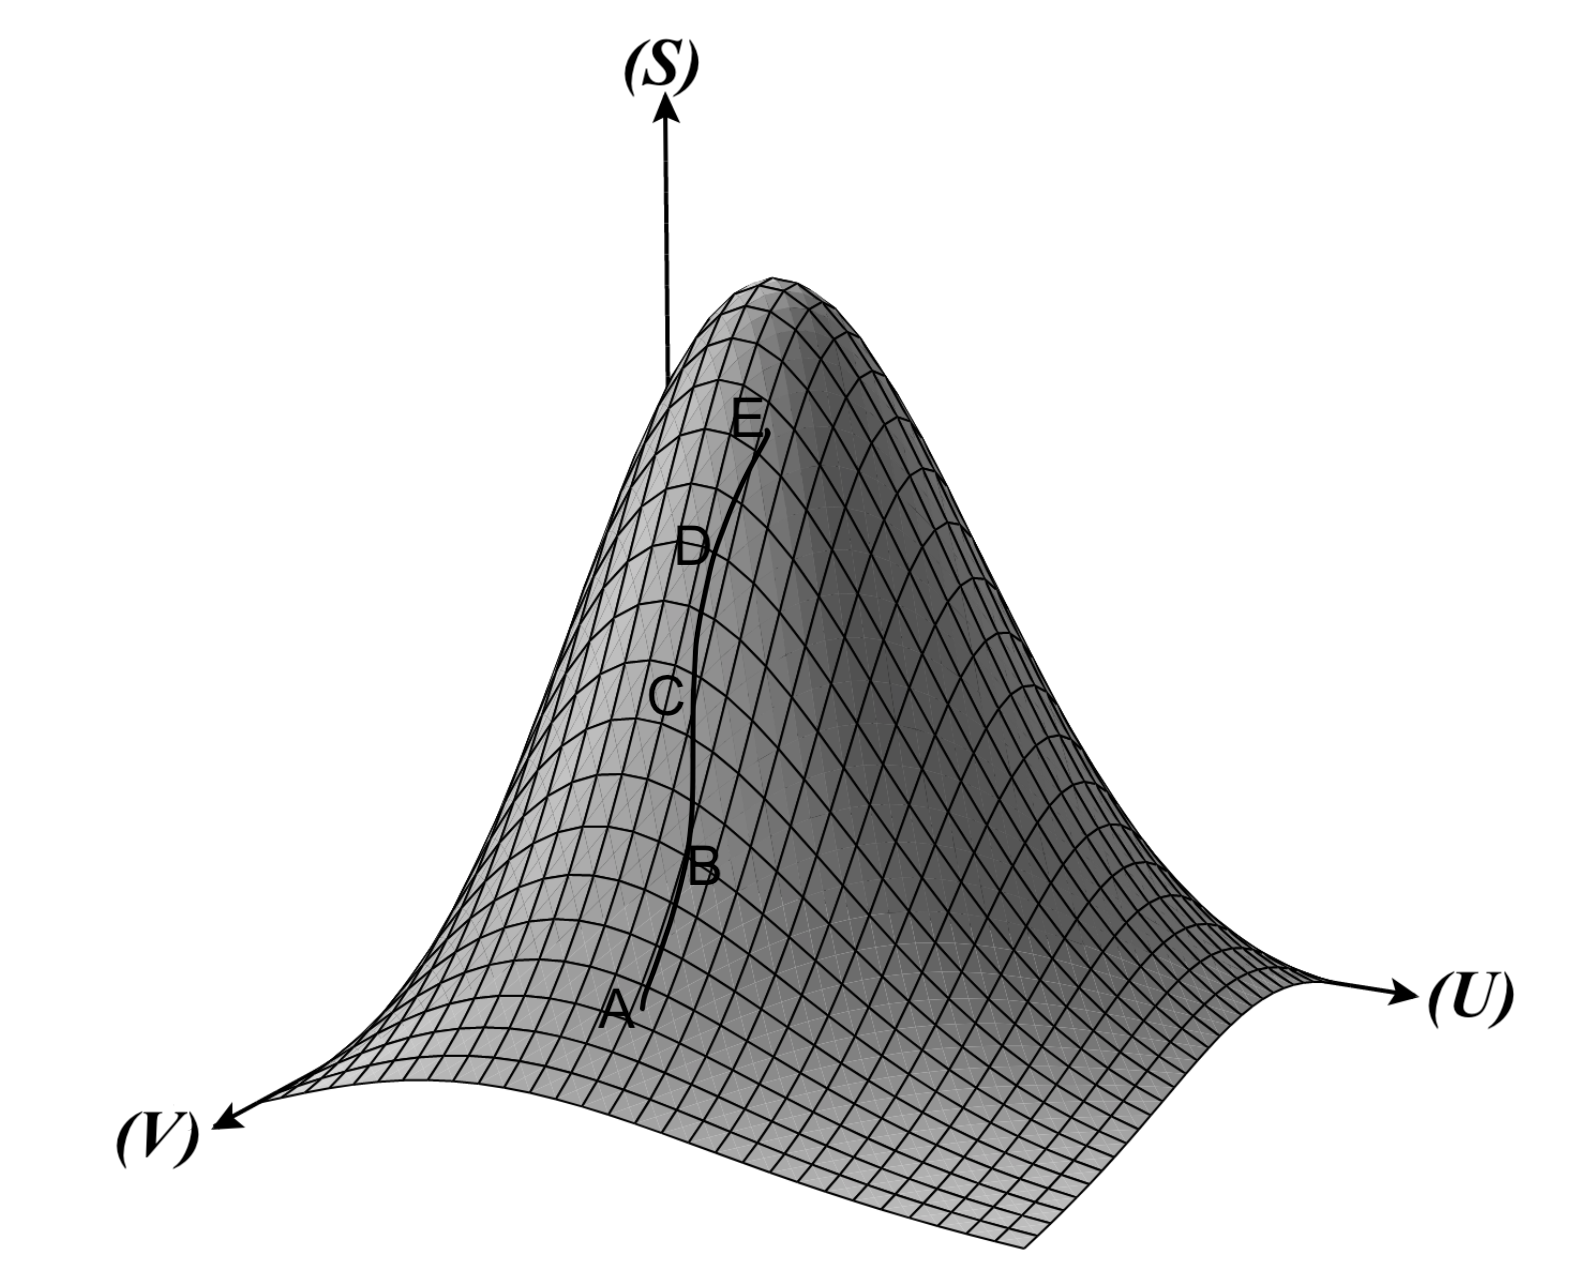
\includegraphics[width = 12cm, height = 8cm]{Curve1}
\end{center}
\begin{center}
Figure 1.1 : A 3-D Surface that represents the curve $S = S(U,V)$ and the process A to E
\end{center}

In this figure, consider any state A, and a process(represented by a succession of states, i.e a one-dimensional curve) that takes it to a final state E. Consider points B,C and D along the way. We achieve this process, by letting go of some constraint to state A so that it spontaneously equilibrates to state B. We repeat this process till we reach E. The limiting case when B $\rightarrow$ A describes a quasi-static process.\\

However, even if B is sufficiently close to A, then letting go of any constraint at B would not make the system go from B to A, because entropy decreases in this process. Only in the hypothetical (and physically unachievable) limit when B $\rightarrow$ A can it go 'backwards', i.e in the direction of decreasing entropy. The one-directional nature of the process A to B, when A and B are not sufficiently close, makes the process \emph{irreversible}.

\begin{mdframed}[style=exercise]
\textbf{Definition 1.9}
 \\*Irreversible process: A real process which is an approximation of a quasi-static locus, in which the entropy monotonically increases, is called an irreversible process. \\ 
\end{mdframed}

\begin{mdframed}[style=exercise]
\textbf{Definition 1.10}
 \\*Reversible process: A real process in which the increase in entropy tends to zero, is called a reversible process. \\ 
\end{mdframed}

Figure 1.2 contains the surface-representation of a reversible process from state A to state E.\\

\begin{center}
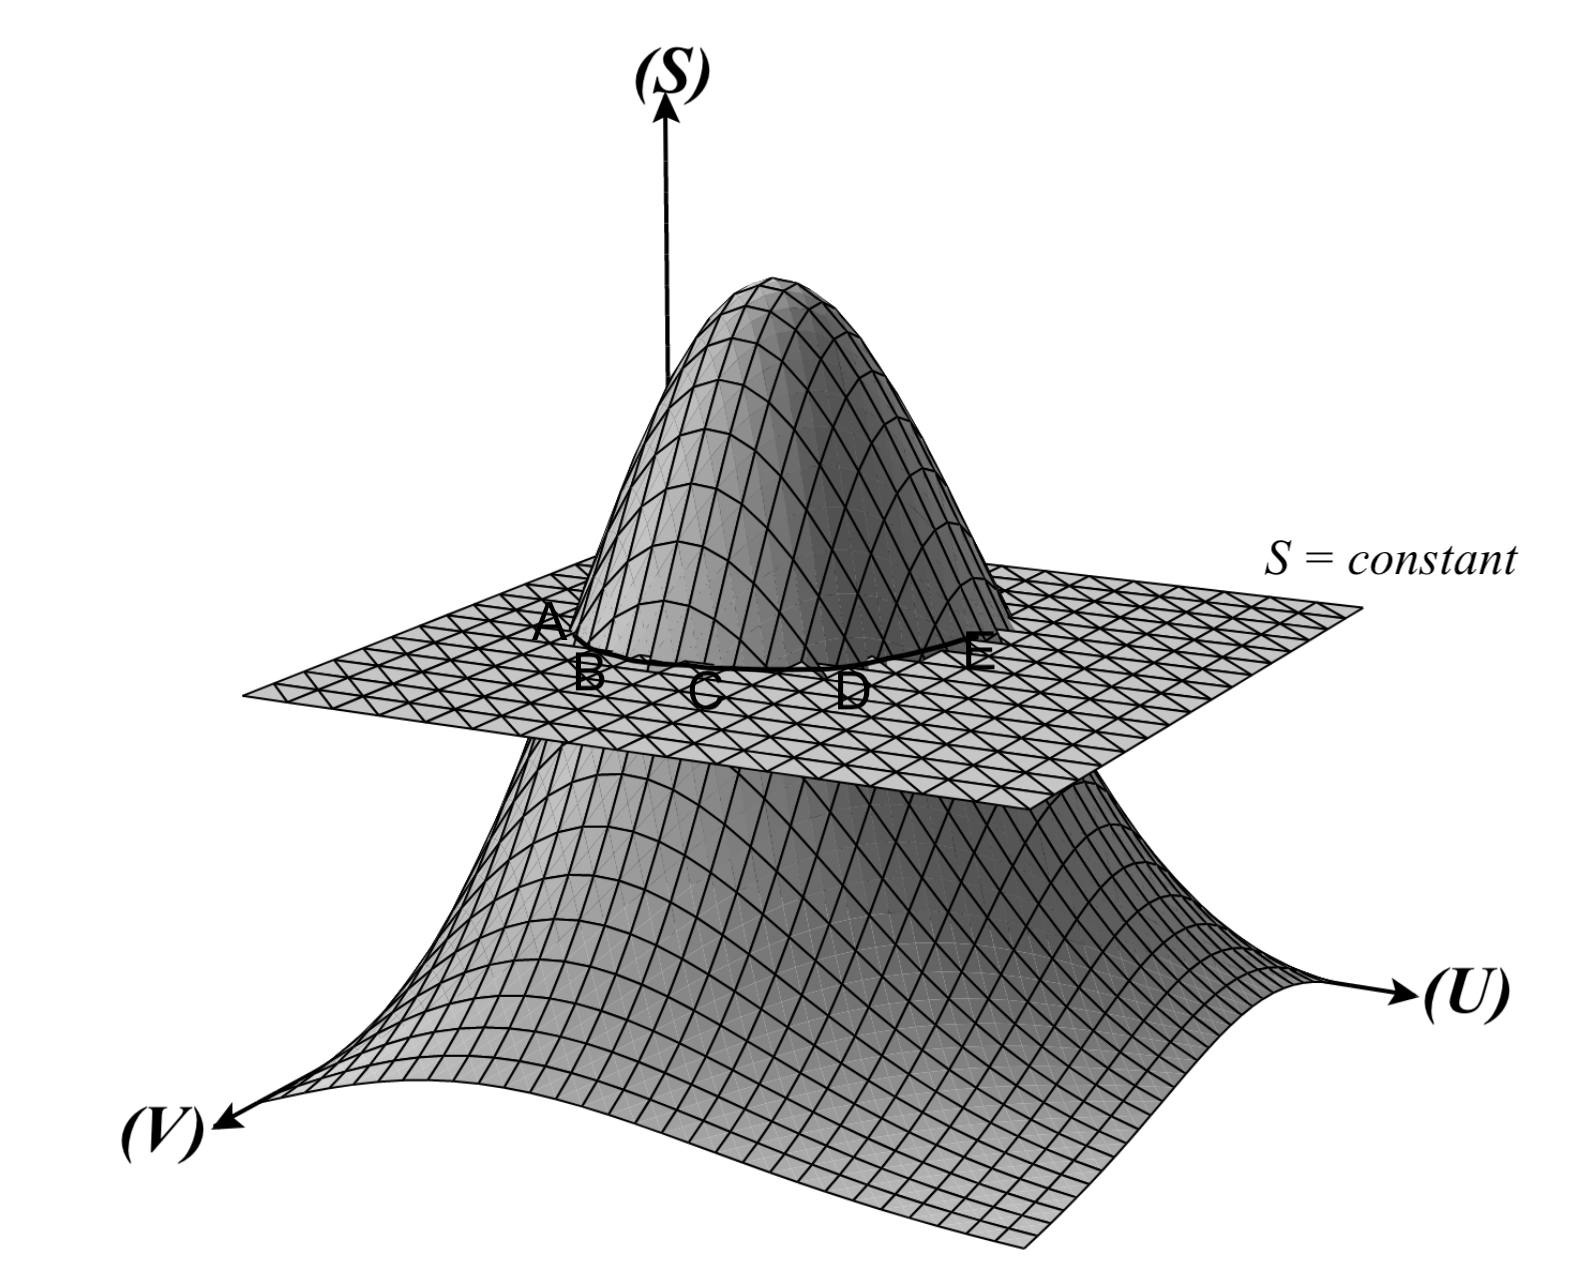
\includegraphics[width = 12cm, height = 8cm]{Curve2}
\end{center}
\begin{center}
Figure 1.2 : A 3-D Surface that represents the curve $S = S(U,V)$ and a reversible process A to E 
\end{center}

A famous 'though-experiment' that helps us to visualise a reversible process is to imagine a gas in a container with a movable piston on top. The piston has a heap of sand on it, and removing one grain of sand would still cause the system to be in equilibrium with the previous state. We slowly remove grain by grain, and this constitutes a reversible process, as we can reverse it by adding a grain of sand back at any time. Similarly, for any, a reversible process, we let go of some minor constraint, and let the system achieve equilibrium in this \emph{slightly modified} state. However, we must wait for \emph{some time} for this system to achieve equilibrium. This \emph{time} is quantified below:

\begin{mdframed}[style=exercise]
\textbf{Definition 1.11}
 \\*Relaxation Time of a System: The time which a system takes to attain equilibrium when a slight constraint has been relaxed, is called the relation time of the system. \\ 
\end{mdframed}

\section{Heat and Work}
\begin{mdframed}[style=exercise]
\textbf{Definition 1.12}
 \\* The reversible work done for any reversible process (in which mole numbers do not change) is equivalent to the mechanical work done on the system. It may be identified as
\[ \eth W = -PdV\]
\end{mdframed}

\begin{mdframed}[style=exercise]
\textbf{Definition 1.13}
 \\* The reversible heat flux for any reversible process (in which mole numbers do not change) is defined as the change in internal energy during the process, diminished by the work done during the process. 
\[ \eth Q = dU - \eth W\]
\end{mdframed}

A few points to be noted:
\begin{enumerate}
    	\setcounter{enumi}{0}
		\item If the internal energy decreases in any process, $dU$ is taken as negative. If work is done on a system, it is taken as positive work. The sign convention for heat flux follows from this.
	\item We have defined work done and heat flux only for reversible processes.
	\item Heat flux is a process of exchanging energy, just like work, and is not a form of energy in itself. This is indicated by writing $\eth Q$ and $\eth W$ instead of $dQ$ and $dW$. Therefore, it makes no sense to ask, "What is the heat content of this system?", this question is as meaningless as, "What is the work done present in the system?".
	\item The power of this definition of heat flux, stems from the fact that we can never truly know the total internal energy of a system. Let us say, we carry out a process by doing some work on the system. We then observe the change in internal energy of the system. The work done may not be equal to the change in the internal energy, because we have defined internal energy only by considering a finite set of contributors to the energy. We may have included the translational kinetic energy energy of every molecule, but not the quantum rotational or vibrational levels of every molecule. Where does the remainder of the energy used in doing the work go? The simplicity of this definition allows us to say, that the remainder of this energy (put in doing work), that does not directly manifest as measurable energy, is the heat flux associated with the system. 
	\end{enumerate}	
	
	\begin{mdframed}[style=exercise]
\textbf{Definition 1.14}
 \\* An adiabatic wall is a constraint seperating two systems that does not allow transfer of energy between the two, by any mechanism.
\end{mdframed}

\section{The Maximum Work Theorem}

	\begin{mdframed}[style=exercise]
\textbf{Definition 1.15}
 \\* A Reversible Work Source(RWS) is a system enclosed by adiabatic walls, impermeable to matter flow, with a relaxation time so small that essentially all processes within it are effectively quasi-static.
\end{mdframed}
In practice, a reversible work source is a frictionless mechanical system which interacts with the rest of the universe only through mechanical work done. For a RWS, we shall be using the symbols $dW$ and $\eth W$ interchangeably. A very large RWS is often called a 'Reservoir'. The atmosphere is an example of a 'Pressure Reservoir'.

	\begin{mdframed}[style=exercise]
\textbf{Definition 1.16}
 \\* A Reversible Heat Source (RHS) is a system enclosed by rigid(immovable) walls, impermeable to matter flow, with a relaxation time so small that essentially all processes within it are effectively quasi-static. 
\end{mdframed}
No work can be done on a reversible heat source. If an RHS is at temperature $T$, then in a given process the change in its internal energy and entropy are related as $dU = TdS = \eth Q$. Due to this equality, for an RHS, we shall be using the symbols $dQ$, $dU$ and $\eth Q$ interchangeably, and shall call the heat flux to an RHS as the heat given to the RHS.\\

 A reversible heat source can be thought of as an ocean at a constant temperature; adding a bucket of hot or cold water will not change its temperature but will only change its internal energy. Thus, an RHS is sometimes called 'a Heat Reservoir'. \\

We shall now be stating, what is known as the \textbf{Maximum Work Theorem}.
	\begin{mdframed}[style=exercise]
\textbf{Theorem 1.1}
 \\* Among all processes leading from an initial state to a final state of a primary system, the work delivered to a secondary system is maximum(and simultaneously, the heat delivered is minimum) for a process that is reversible.
 \end{mdframed}
 
\textbf{Proof} Consider a primary system that goes from $S_1(U_1,V_1,N_1,....)$ to $S_2(U_2,V_2,N_2,....)$. Consider two routes that the system can take to achieve this transition. For both the routes, $\Delta S_{primary}$ and $\Delta U_{primary}$ are the same. Consider that along both these routes, the primary system is connected to a RWS and an RHS as in Figure 1.3.\\ 
%Figure 1.3
\begin{center}
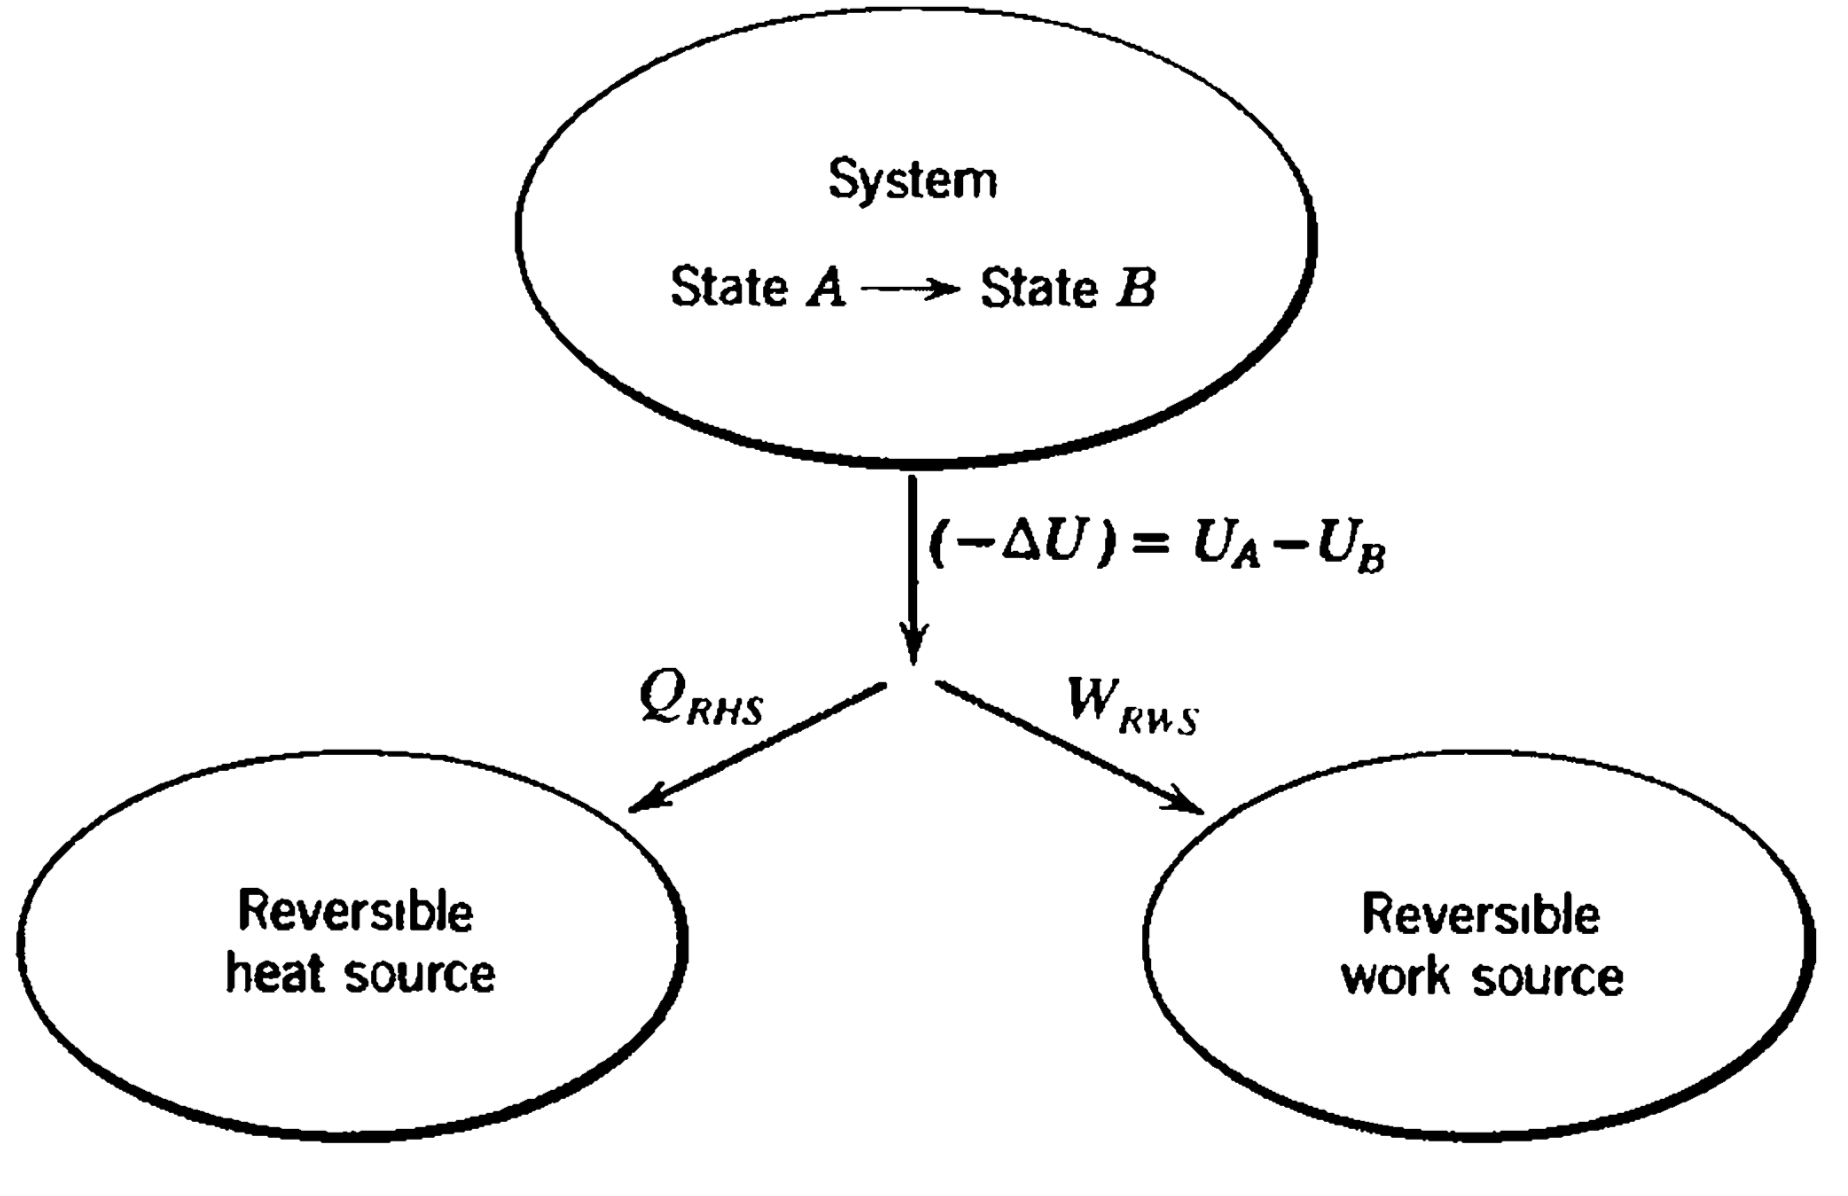
\includegraphics[width = 9cm, height = 4cm]{Work}
\end{center}
\begin{center}
Figure 1.3 : A schematic representation of the process as described in the proof of the Maximum Work Theorem\\
(taken from \emph{Thermodynamics and an Introduction to Thermostatistics} by Herbert B. Callen)
\end{center}


It is evident that the two processes differ only in the ratio of Work Done on RWS and Heat given to RHS. Energy conservation requires that

\[ \Delta U_{primary} + W_{RHS} + Q_{RHS} = 0 \]

The entropy maximum postulate requires that 

\[ \Delta S_{net} = \Delta S_{primary} + \Delta S_{RHS}  = \Delta S_{primary}  + \frac{Q_{RHS}}{T_{RHS}} \geq0 \]

Combining the two equations, we obtain

\[ W_{RHS} \leq T_{RHS} \Delta S_{primary} - \Delta U_{primary} \]

For the maximisation of work, we take the equality, which gives us $\Delta S_{net} = 0$, i.e the process must be reversible.

	\begin{mdframed}[style=exercise]
\textbf{Corollary}
 \\* The delivery of work and heat are identical for every reversible process.
 \end{mdframed}
 
 Let us now calculate the maximum work that can be delivered to the RWS. Using the definition of heat, we have $Q_{RHS} = \Delta U_{primary} - W_{primary} $
 
 \[ W_{RHS} = T_{RHS} \Delta S_{primary} - \Delta U_{primary} \]
 \[= T_{RHS} \frac {Q_{RHS}} {T_{primary}} - \Delta U_{primary} \]
 \[= T_{RHS} \frac {Q_{RHS}} {T_{primary}} - Q_{RHS} - W_{primary} \]
 \begin{center}
  \boxed{= (-Q_{RHS})\Bigg(1 - \frac {T_{RHS}} {T_{primary}}\Bigg) + (- W_{primary}) }
  \end{center}
  
\vspace{1cm}
This leads to another corollary: 
	\begin{mdframed}[style=exercise]
\textbf{Corollary}
The maximum work delivered to the RWS is the sum of
\begin{enumerate}
    	\setcounter{enumi}{0}
	\item The work ($-W_{primary}$) extracted directly from the system
	\item The fraction $ \Bigg(1 - \frac {T_{RHS}} {T_{primary}}\Bigg) $ of the heat ($-Q_{RHS}$)directly extracted from the system(i.e the heat delivered to RHS)
\end{enumerate}
 \end{mdframed}

\section{Engines, Refrigerators, Pumps}
We shall consider three specific machines that operate on the principle of the last corollary. Each of these involves a 'hot' subsystem at high temperature $T_h$, and a 'colder' RHS at temperature $T_c$. Work is delivered to a RWS. All the efficiencies are simply measures of performance, derived using the last corollary. 
\begin{enumerate}
    	\setcounter{enumi}{0}
	\item \textbf{The Engine}\\
	In this case the 'hot' subsystem is a furnace or a boiler, the 'cold' subsystem may be the ambient atmosphere. The measure of performance is the fraction of the quantity of heat $(-Q_{RHS})$ withdrawn from the hot RHS, converted to work $W_{RWS}$. We take $W_{primary}$ to be zero, because it is simply additive to the work delivered, and obtain the efficiency of the engine as
	\[\eta = \Bigg(1 - \frac {T_{c}} {T_{h}}\Bigg) \]
	%Figure 1.4
	\begin{center}
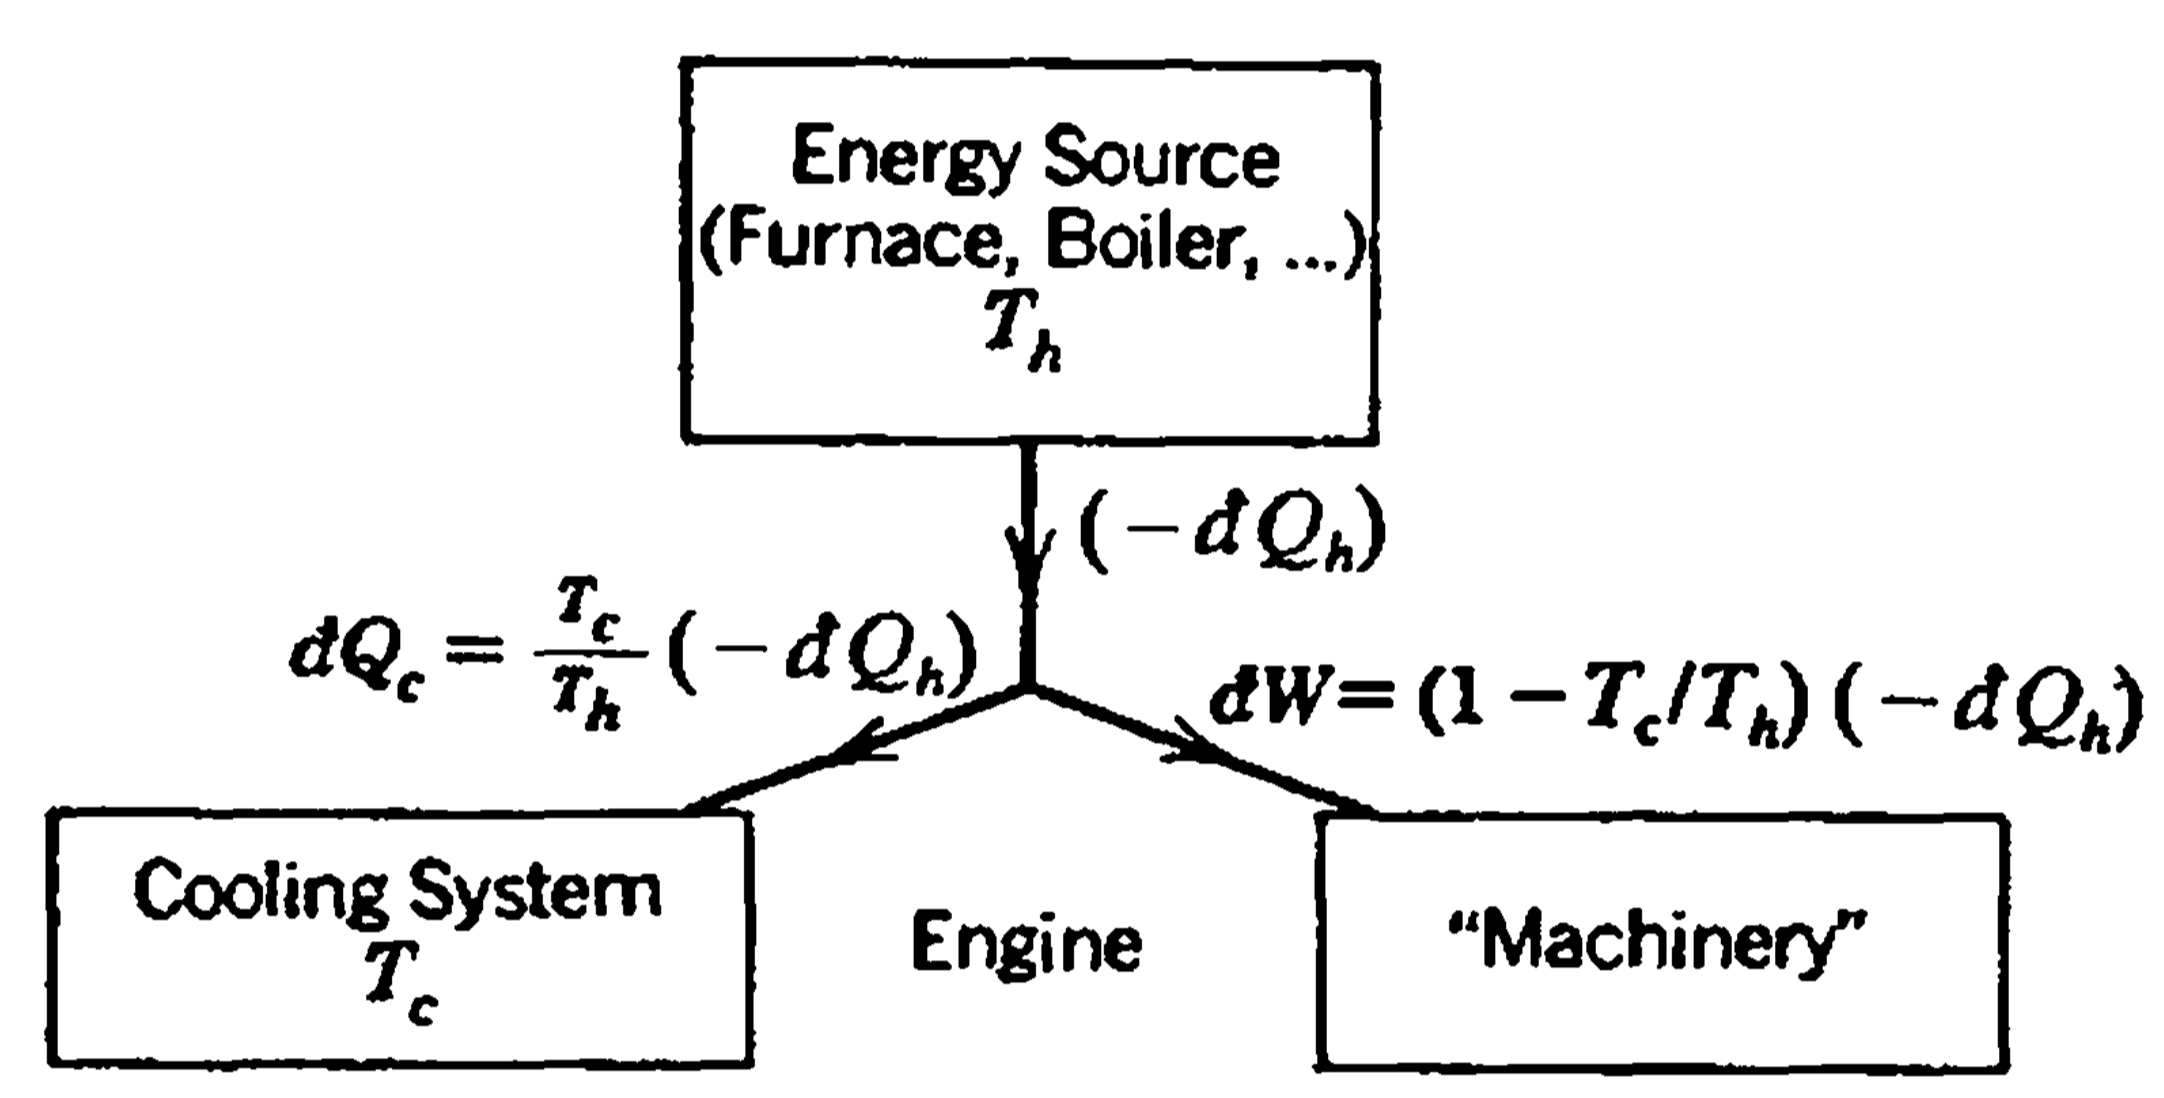
\includegraphics[width = 9cm, height = 4cm]{Engine}
\end{center}
\begin{center}
Figure 1.4 : A schematic representation of a Thermodynamic Engine\\
(taken from \emph{Thermodynamics and an Introduction to Thermostatistics} by Herbert B. Callen)
\end{center}
	An important way of realising the Thermodynamic Engine is to make a gas go through what is called the \textbf{Carnot Cycle}. A gas is the 'working part' in this cycle, and it is taken through a $P-V$ Cycle as shown below:\\
	%Figure 1.5\\
	\begin{center}
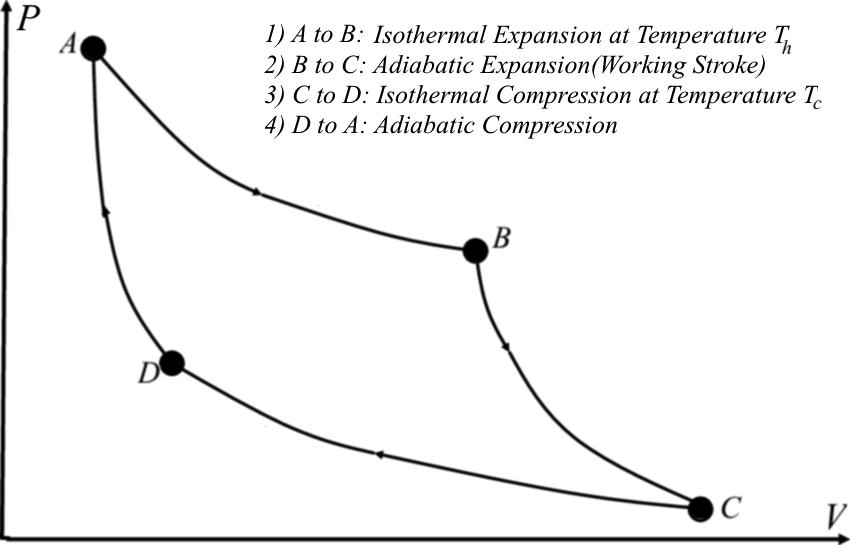
\includegraphics[width = 10cm, height = 5cm]{PV}
\end{center}
\begin{center}
Figure 1.5 : A P-V Diagram of a Carnot Cycle\\
\end{center}
	A typical Carnot Engine has an efficiency of around 0.3. This is due to friction losses, and due to the fact that no process is slow enough to be quasi-static. However, even if these limitations could be overcome, the maximum efficiency is still capped by thermodynamic laws, and this is a direct consequence of the Entropy Maximum Postulate. More discussions on this will be made in Chapter 3.
	\item \textbf{The Refrigerator}\\ 
	In a refrigerator, heat is extracted from a cold system, with the input of minimum amount of work, to eject heat into the comparitively hot ambient atmosphere. The efficiency is the ratio of the heat removed from from the cold system to the work that must be put in to cool it further, i.e
	\[\eta = \frac {(-Q_c)} {(-W_{RWS})}  = \Bigg(\frac {T_{c}} {T_h-T_c}\Bigg) \]
	%Figure 1.6
	\begin{center}
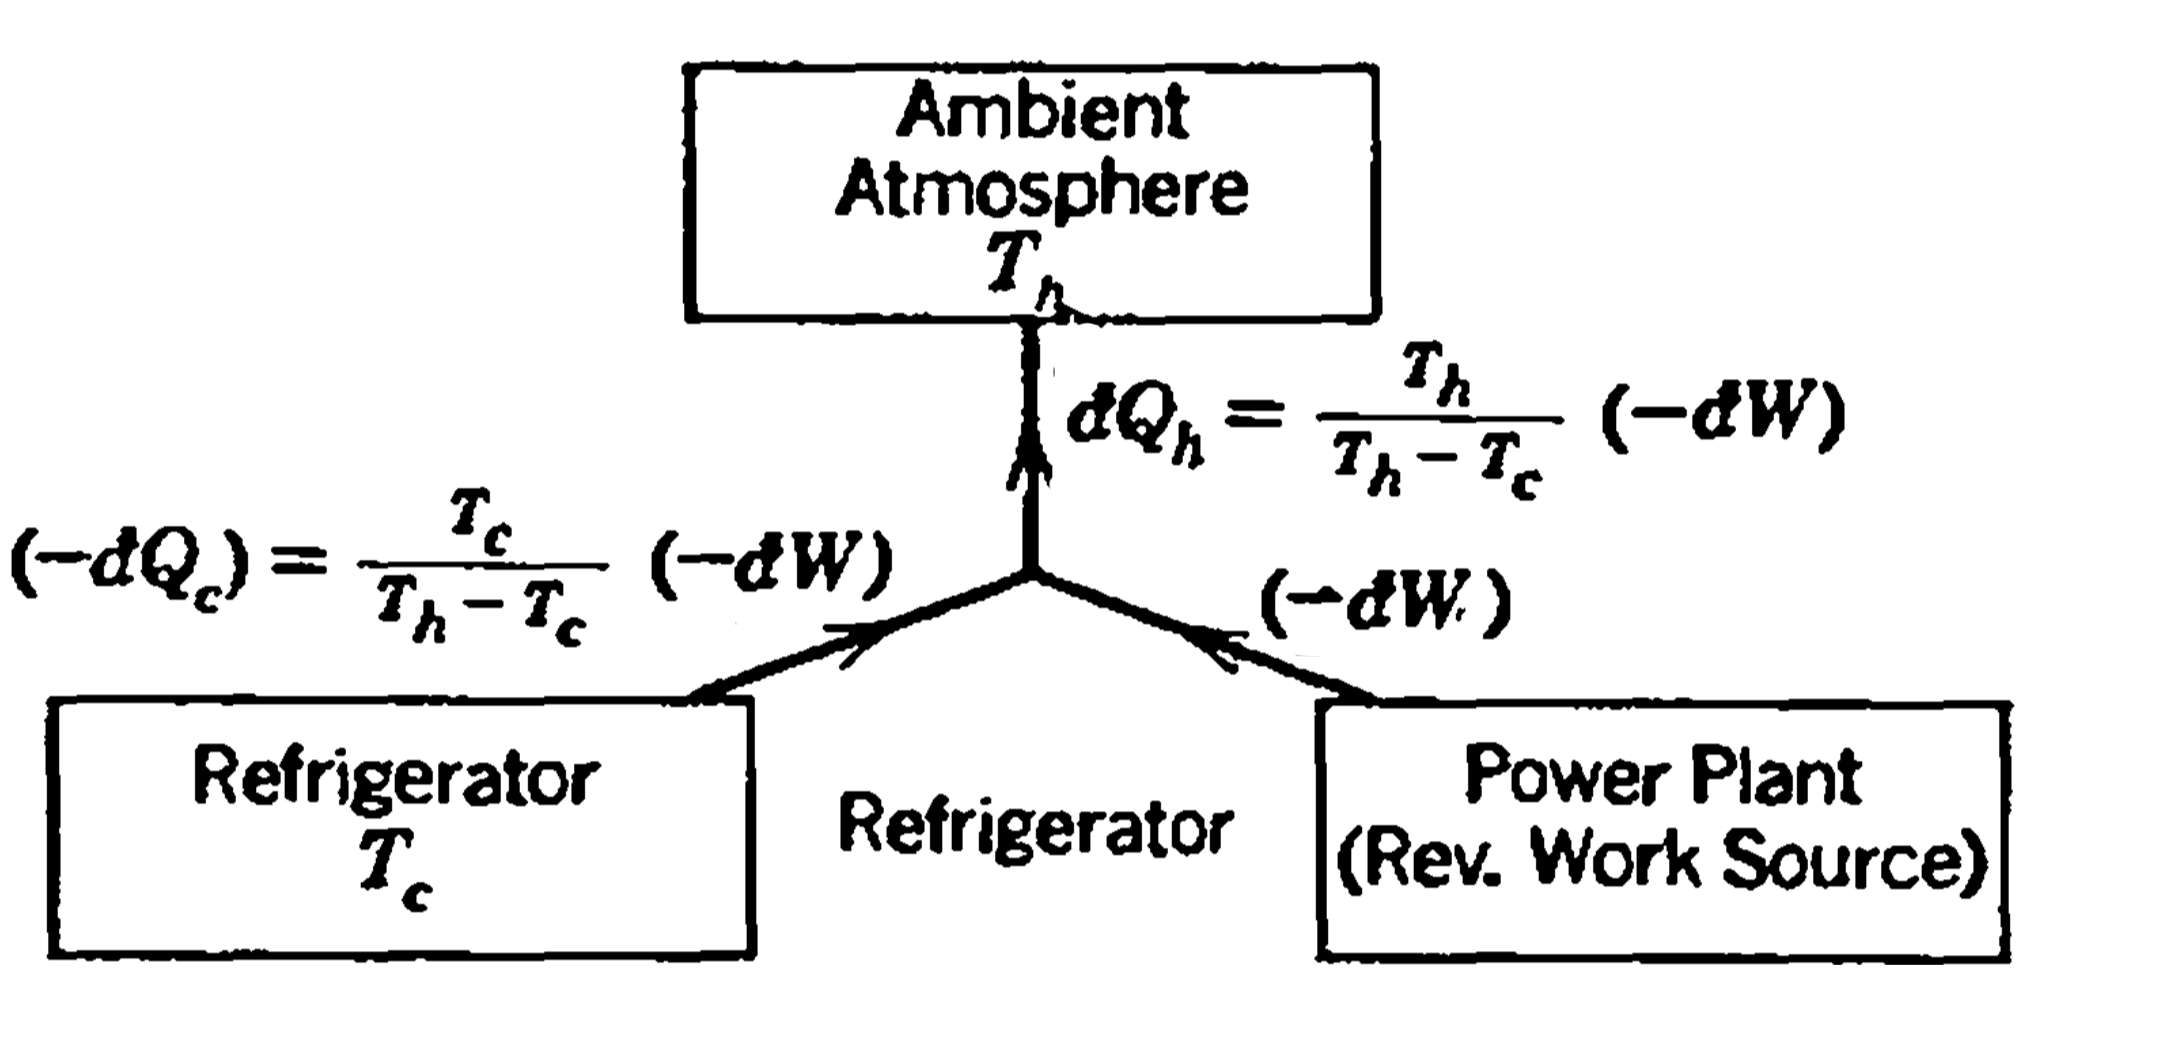
\includegraphics[width = 9cm, height = 4cm]{Fridge}
\end{center}
\begin{center}
Figure 1.6 : A schematic representation of a Thermodynamic Refrigerator,\\
(taken from \emph{Thermodynamics and an Introduction to Thermostatistics} by Herbert B. Callen)
\end{center}
	\item \textbf{The Pump}
	A pump is the same as a refrigerator, it is just that its purpose is not to cool the cold system, but to heat the hotter system. The efficiency is the ratio of the heat delivered to the hot system to the work extracted from the RWS.
	\[\eta = \frac {(Q)} {(-W_{RWS})}  = \Bigg(\frac {T_{h}} {T_h-T_c}\Bigg) \]
	\end{enumerate}
	
\section{The Energy Minimum Principle}
It is easy to observe from Postulate II the invertibility of the equation $S = S(U,V,N....)$. This means that we can write $U = U(S,V,N,...)$ and use this as our equation of state. The question is, what is the equivalent of the Entropy Maximum Postulate in this inverted representation? The answer is the \emph{Energy Minimum Principle}, which states that "the values that unconstrained parameters of a system attain at equilibrium are those that minimise the total energy of the system, with the total entropy of the system being held constant." 
\\ 
\\
\textbf{Proof} Consider a system with $S = S(U,X)$. At equilibrium, we have
 \[\frac{\partial S}{\partial X} = 0 \hspace{0.5cm}and \hspace{0.5cm}\frac{\partial ^2 S}{\partial ^2 X} < 0 \] 
 Using the chain rule for partial derivatives, we conclude that $U$ has an extremum based on the following: 
 \[ \frac{\partial U}{\partial X} = - \frac  {\Big(\frac{\partial S}{\partial X }  \Big)} {\Big(\frac{\partial S}{\partial U }         \Big)}  = -T\frac{\partial S}{\partial X} = 0 \]
 We now conclude that this extremum is a point of minima based on the following:
  \[ \frac{\partial ^2 U}{\partial X^2} = \frac{\partial }{\partial X} \Bigg[- \frac  {\Big(\frac{\partial S}{\partial X }  \Big)} {\Big(\frac{\partial S}{\partial U }  \Big) }  \Bigg]  
= -\frac{ \frac{\partial ^2S} { \partial X^2 }    }{  \frac{\partial S}{\partial U}      } + \Big(\frac{\partial S}{\partial X}\Big)\frac{\frac{ \partial^2S  }{\partial X \partial U}       }{ \big( \frac{\partial S}{\partial U} \big)^2}
  = -T\frac{\partial ^2S}{\partial X^2} > 0 \]
 
The derivation of the Energy Minimum Principle is exactly isomeric to the derivation of the Gibbs Minimum or Enthalpy Maximum principles that we shall encounter in Section 1.11.\\

\section{Other Potentials}
It is in most cases, easier to physically measure intensive quantities like Temperature, Pressure and Chemical Potential. However, an equation of the form $S(T,V,N)$ is \emph{not} an equation of state, as it contains considerably less information than an equation of the form $S(U,V,N)$. If we have an equation of state in the extensive parameters, we could differentiate it to obtain the intensive parameters. Is the reverse true? We could, using the equation $f(S,T,V,N) = 0$ express $T$ in terms of $S$ and $N$ and come up with something like  $T = \frac{\partial U}{\partial S} = g(S,V,N)$. Integration of this equation is not easy and even if it were, it would not give us $U$, as we would have \emph{no way} of knowing the integration constant. However, an equation of state should be all-encompassing, and should contain \emph{all} the information regarding a system. Thus we can be sure that an equation of state can't involve intensive parameters. How, then, are we to deal with systems where it is only possible to measure the intensive parameters?\\

The trick is to use a \emph{Legendre transform} of the Entropy.\\

Consider a simple case in which the entropy is a function of one extensive parameter $E$, i.e $S = S(E)$. Let the intensive parameter $I$ be $I = \frac{dS}{dE}$. Now, we shall create a \emph{new} function of the intensive parameter $\psi = \psi(I)$, and we will construct back the original function $S = S(E)$ from $\psi = \psi(I)$. The trick is, that \emph{we define} $\psi$ in such a way that "For any point on the curve $S = S(E)$, the S-intercept of the tangent (having slope $I$) at any point $(E,S)$ is $\psi(I)$".\\

Once we define a $\psi$ in this way, all we have to do is take many readings of $I$ and for every $I$ calculate $\psi(I)$. Then we draw a graph of $S$ vs $E$ with the following rule: we draw an infinite number of tangents, each having a different slope $I$, and an intercept $\psi(I)$. The envelope of this family of lines gives us the graph of $S = S(E)$.\\

In this case, $\psi(I)$ is called the \emph{Legendre transform} of the function $S(E)$.\\

We shall be defining four popular Legendre transforms of entropy that operate on exactly the same principle. Each of the transforms defined below is called a 'Potential', and contains exactly the same amount of information as the entropy equation of state. They are not 'different quantities' and are most certainly not 'lesser' in any way to the entropy. It is just that it is easier to deal with these potentials in certain cases, as compared to the entropy, both physically(as far as measuring quantities is concerned) and mathematically. Just as there is an Entropy Maximum Postulate, there are equivalent principles that involve maximisation/minimisation of the potentials, and these have the same physical significance as entropy maximisation. A person who deals with the Gibbs Potential,  should not have to transform his/her equation to the entropy representation and then maximise it, he/she should be able to directly use the principle that deals with the Gibbs Potential.
\\

\begin{enumerate}
    	\setcounter{enumi}{0}
	\item \textbf{The Helmholtz Potential}
		\begin{mdframed}[style=exercise]
\textbf{Definition 1.16}
 \\* The Helmholtz Potential$(F)$ is the partial Legendre transform of of the equation $U = U(S,V,N....)$ that replaces the entropy by the temperature as the independent variable. The equation of the form $\psi = \psi(I)$ for it is 
 \[F = U - TS\]
\end{mdframed}
\textbf{The Helmholtz Minimum Principle} (corresponding to the Entropy Minimum Principle) is that the equilibrium value of any unconstrained internal parameter in a system in contact with a heat resevoir is the one that minimises the Helmholtz Potential over the manifold of states for which $T = T_r$.

	\item \textbf{The Enthalpy}
	\begin{mdframed}[style=exercise]
	\textbf{Definition 1.16}
 \\* The Enthalpy $(H)$ is the partial Legendre transform of of the equation $U = U(S,V,N....)$ that replaces the volume by the pressure as the independent variable. The equation of the form $\psi = \psi(I)$ for it is 
 \[H = U + PV\]
\end{mdframed}
\textbf{The Enthalpy Minimum Principle} is that the equilibrium value of any unconstrained internal parameter in a system in contact with a pressure reservoir(most often, the atmosphere), is the one that minimises the Enthalpy over the manifold of states for which $P = P_{atm}$.\\
Since $ H = U + PV $, and when the system is in contact with a pressure reservoir, we have $dH = dU + PdV = \eth Q$, and therefore enthalpy is commonly called the 'heat flux at constant pressure'. The Enthalpy representation is most commonly used in cases where a chemical reaction is carried out in an open vessel.

	\item \textbf{The Gibbs Potential}
	\begin{mdframed}[style=exercise]
		\textbf{Definition 1.16}
 \\* The Gibbs Potential $(G)$ is the partial Legendre transform of of the equation $U = U(S,V,N....)$ that replaces simultaneously the entropy by the temperature, and the volume by the pressure,  as the independent variables. The equation of the form $\psi = \psi(I)$ for it is 
 \[G = U + PV -TS\]
\end{mdframed}
\textbf{The Gibbs Minimum Principle} is that the equilibrium value of any unconstrained internal parameter in a system in contact with a thermal and pressure reservoir is the one that minimises the Gibbs Potential over the manifold of states for which $P = P_{atm}$ and $T = T_{atm}$.\\
The Gibbs representation is extremely powerful for determining the spontaneity of process taking place in a system surrounded by a medium(be it the atmosphere, or a fluid), where temperature and pressure are constant. We can be sure that if in such a scenario $dG<0$, the process will be spontaneous. Also, $U + PV = H$ allows us to recast the Gibbs Potential in the familiar form $G = H - TS$. Just like the the Energy Minimum Principle, the Gibbs Minimum Principle is another physically convenient 'avatar' of the Entropy Maximum Postulate. 

	\item \textbf{The Grand Canonical Potential}
	\begin{mdframed}[style=exercise]
			\textbf{Definition 1.16}
 \\* The Grand Canonical Potential $(\Psi)$ is the partial Legendre transform of of the equation $U = U(S,V,N....)$ that replaces simultaneously the entropy by the temperature and the mole numbers by the chemical potentials, as the independent variables. We have
 \[\Psi = U - TS - \sum_{j = 1}^{r} \mu_j N_j = -PV\]
\end{mdframed}	
\end{enumerate}

\section{Le-Chatelier's Principle}
From the Entropy Maximum Postulate, an equilibrium point must satisfy two conditions: $dS =0$ \emph{and} $d^2S < 0$. We have mostly used the first condition so far, but the second condition reveals important things about the \emph{stability} of the equilibrium point. Le Chatelier's principle is a general statement that deals with the reaction of a system, in \emph{stable} equilibrium, to \emph{slight} disturbances. \\

Let an infinitesimal fluctuation $dE_1^f$ occur in an extensive parameter $E_1$ of a composite system at equilibrium. Let us consider the change in the intensive parameter $I_1 (= \frac{\partial S}{\partial E_1})$ due to this fluctuation:
\[ dI_1^f =  \frac{\partial I_1}{\partial E_1}dE_1^f\]
There is also a change in intensive paramer $I_2 (= \frac{\partial S}{\partial E_2})$, given by 
\[ dI_2^f =  \frac{\partial I_2}{\partial E_1}dE_1^f\]
Now, post this fluctuation, the system will try to attain a 'new' equilibrium. We denote the response of the extensive parameters to the fluctuation $dE_1^f$ by $dE_i^r$ . We now minimise the total energy isentropicaly:
\[d(U^{original} + U^{response}) = (I_1 - I_1^r)dE_1^r + (I_2 - I_2^r)dE_2^r= dI_1^fdE_1^r + dI_2^fdE_2^r \leq 0\]
This gives us both the terms in the inequality simultaneously less than zero(as they are independent), i.e
\[ \frac{\partial I_1}{\partial E_1}dE_1^fdE_1^r \leq 0 \hspace{0.5cm} and \hspace{0.5cm} \frac{\partial I_2}{\partial E_1}dE_1^fdE_2^r \leq 0\]
Consider the partials $\frac{\partial I_1}{\partial E_1}$  and $\frac{\partial I_2}{\partial E_1}$ . Each of these is positive and the proof of the same is left to the reader as an exercise.(Hint: it arises from the downwards concavity of the total entropy at a stable equilibrium)
Multiplying the first inequality by $\frac{\partial I_1}{\partial E_1}$ and the second one by $\frac{\partial I_2}{\partial E_1}$ gives us
 \begin{center}
  \boxed{ dI_1^fdI_1^r \leq 0 \hspace{0.5cm} and \hspace{0.5cm} dI_2^fdI_2^r \leq 0      }
  \end{center}
  i.e \emph{"The intensive parameters $I_1$ and $I_2$ respond in a way that is opposite in sign to the change induced in them by the fluctuation."} This is the statement of the Le-Chatelier Principle.


\section{Chemical Equilibrium}
Consider a simple composite system consisting of two subsystems connected by a rigid(immovable) wall that allows exchange of energy, and permeability to one type of material($N_i$). This wall is impermeable to all other species $N_j \forall j \neq i$. To find the equilibrium values of $U_1, U_2, N_{j,1} and N_{j,2}$ we proceed as in section 1.4:
\[ dS = \frac{1}{T_1'}dU_1'  - \frac{\mu_{j,1}'}{T_1'}dN_{j,1}' + \frac{1}{T_2'}dU_2' - \frac{\mu_{j,2}'}{T_2'}dN_{j,2}'\]
with \[dU_1' = -dU_2' \hspace{0.7cm} and \hspace{0.7cm} dN_{j,1}' = -dN_{j,2}' \]
Combining these two gives us
\[ dS = \Big(\frac{1}{T_1'} - \frac{1}{T_2'}\Big)dU_1'  - \Big(\frac{\mu_{j,1}'}{T_1'} - \frac{\mu_{j,2}'}{T_2'} \Big)dN_{j,1}' \]
As $dS$ is zero for all $dU_1'$ and $dN_{j,1}'$ (this is equilibrium), we obtain $T_1' = T_2'$, and more importantly
\[ \mu_{j,1}' = \mu_{j,2}' \]
This means that the Chemical Potential is the quantity that 'balances' out at equilibrium, and provides us the direction for matter flow. If $\mu_{j,1} > \mu_{j,2}$, then matter will from subsystem 1 to subsystem 2 till the Chemical Potentials balance out.\\

This is of particular interest as it provides insight into Chemical Equilibrium. Consider a container at temperature $T$, with total energy and volume fixed, in which the following gaseous Chemical Equilibrium is present:
\[  0 \rightleftharpoons \sum v_jA_j \]
Here $v_j$ is the stoichiometric coefficient of the $j^{th}$ species $A_j$. Examples of gaseous reactions written in this notation are $0 \rightleftharpoons O_2 - 2O $ and $0 \rightleftharpoons 2H_2O - 2H_2 - O_2$

We have, at equilibrium,
 \[dS =  - \frac{1}{T}\sum_{j = 1}^{r}\mu_jdN_j = 0\]
 Noting that $dN_j$, i.e the change in number of moles of the $j^{th}$ component is directly proportional to the stoichiometric coefficient $v_j $, we obtain a powerful relation
 \begin{center} \boxed{\sum_{j = 1}^{r}\mu_jv_j = 0}\end{center}
 Also, for a multi-component mixture of ideal gases, we have the (easily derivable, as in Example. 1.1) equations:
\[S = \sum_{j}^{}N_js_{j0} + R\Bigg(\sum_{j}^{}N_jc_{j}\Bigg)\ln \Bigg(\frac{T}{T_0}\Bigg) + R\sum_{j}^{}N_j \ln \Bigg(\frac{V}{N_jv_0}\Bigg)\]
and
\[U = RT\Bigg(\sum_{j}^{}N_jc_{j}\Bigg)\]
We calculate, using these equations, the Chemical Potential of the $j^{th}$ component, which is in most general terms given by:
\[ \mu_j = \frac{\partial U}{\partial N_j}  = RT\bigg[\phi_j(T) + \ln P + \ln (\chi_j) \bigg] \]
Here $\phi_j(T)$ is purely a function of the Temperature, $P$ is the total pressure, and $\chi_j$ is the mole fraction of the $j^{th}$ component. Combining with $\sum\mu_jv_j = 0$ gives us 
\[ \sum_{j }^{}v_j\ln (\chi_j) = -\sum_{j}^{}v_j \ln P - \sum_{j}v_j\phi_j(T) \]

We \emph{define} the \textbf{Equilibrium Constant} $\bm{K(T)}$ of a reaction as
\begin{center}
\boxed{ \ln K(T) =  \sum_{j}v_j\phi_j(T)}
\end{center}

This gives us the incredibly important \textbf{Mass Action Law}:
\begin{center}
\boxed{ \prod_{j}^{}\chi_j^{(v_j)} = P^{(\Sigma v_j)}K(T) }
\end{center}
The Mass Action Law is an incredibly powerful formulation that forms one of the tenets of Theoretical Chemistry. This formulation not only validates the algorithms used for solving for equilibrium related problems, but can be expanded to a wide range of phenomena involving non-homogenous chemical equilibria.
%%%%%%%%%%%%%%%%%%%%%%%%%%%%%



























%%%%%%%%%%%%%%%%%%%%%%%%%%%%%
\chapter{Statistical Mechanics}
\section{The predictive nature of Statistical Mechanics}
In this chapter, we shall be doing the same thing that we did phenomenologically - given an initial state of a system, we shall attempt to predict the final state that the system will evolve to. However, unlike the phenomenological approach, we shall not be defining any postulates. We shall be taking this task of prediction \emph{literally},  and we shall do so by involving probabilities.\\

Before going into the details, it is worth mentioning 'macrostates' and 'microstates'. Usually, the macroscopic state of a system (Definition 1.4)  is called a macrostate. Quantum mechanics tells us that each macrostate can consist of numerous 'microstates' that the system can be in. Two different systems can thus be in the same macrostate, but different microstates.\\

The way statistical mechanics works is this: we are given a system in some initial state(macro or micro). We then let go of some constraints that allow the system to possibly occupy other states(macro or micro). We then 'predict' that the system in these given conditions can occupy all of the states(macro or micro) $x_1,x_2,x_3,...,x_n$, with the probability of occupation of each state being $p_1,p_2,p_3,....,p_n$.\\

What does 'probability of occupation' mean? It can have two definitions. The first definition, which was given by Boltzmann, states that the probability of occupation of a state is the fraction of time that the system spends in that state. As far as this text is concerned, this definition holds good. However, it does lead to problems in some cases, which leads us to the newer definition.\\

\begin{mdframed}[style=exercise]
\textbf{Definition 2.1}
 \\* We imagine a large array of identical copies of a system. We define the probability of the system being in a state as the fraction of the array that is in that state.
 \end{mdframed}
 
Thus, in statistical mechanics, if we are able to figure out the probability of occupation of each state, we are done. However, we are not using any postulate that provides us with the algorithm to compute the probability distribution of the various states that a system can occupy. What we use is a guiding principle, that in essence, says: \emph{"We don't know what state the system will be in"}

\section{Uncertainty, Disorder and Entropy}
Consider a die being thrown. If asked to predict, what face will show up, one can predict anything. A person may say with confidence, that the number 'six' will definitely show up, and no other number will. A second person may say that each of the six numbers has an equal probability of appearing. A third person may say that the die may be biased, and that each number has an associated probability of appearing.\\

The question is, out of all these three predictions, which is the most \emph{natural} one?
\begin{enumerate}
\item Clearly, the first prediction is the most unscientific. In our strategy of prediction, we want to avoid unreasonable bias to any one state.
\item However, assuming that each number has equal probability, is to say that the die is unbiased in all cases. We want a strategy of prediction that allows for inclusion of bias.
\end{enumerate}

Consider another set of two predictions: A person 'P' says that the numbers 3 and 4 will appear with probability 0.5 and 0.5. A person 'Q' says that the numbers 2, 5 and 6 will appear with probability of 0.2, 0.3 and 0.5 respectively. Why is it that we intuitively feel that person Q's prediction is more \emph{fairer}?\\

The answer is that Q's probability distribution has a greater 'uncertainty' associated with it, and any probability distribution that is 'certain', \emph{seems} like an unfair and unreasonable prediction, because both the people have the same information before making their prediction.

\begin{mdframed}[style=exercise]
\textbf{Definition 2.2}
 \\* The uncertainty $(\delta)$ associated with a discrete probability distribution consisting of discrete random variables $x_1,x_2,x_3,...,x_n$ with associated probabilities $p_1,p_2,p_3,....,p_n$ is given by
 \[ \delta = -k\sum_{i= 1}^{n}p_i\ln(p_i) \]
 where $k$ can be any real number.
 \end{mdframed}
 
Given below are a few discrete probability distributions. 

%%%gRAPHIC END

\begin{center}
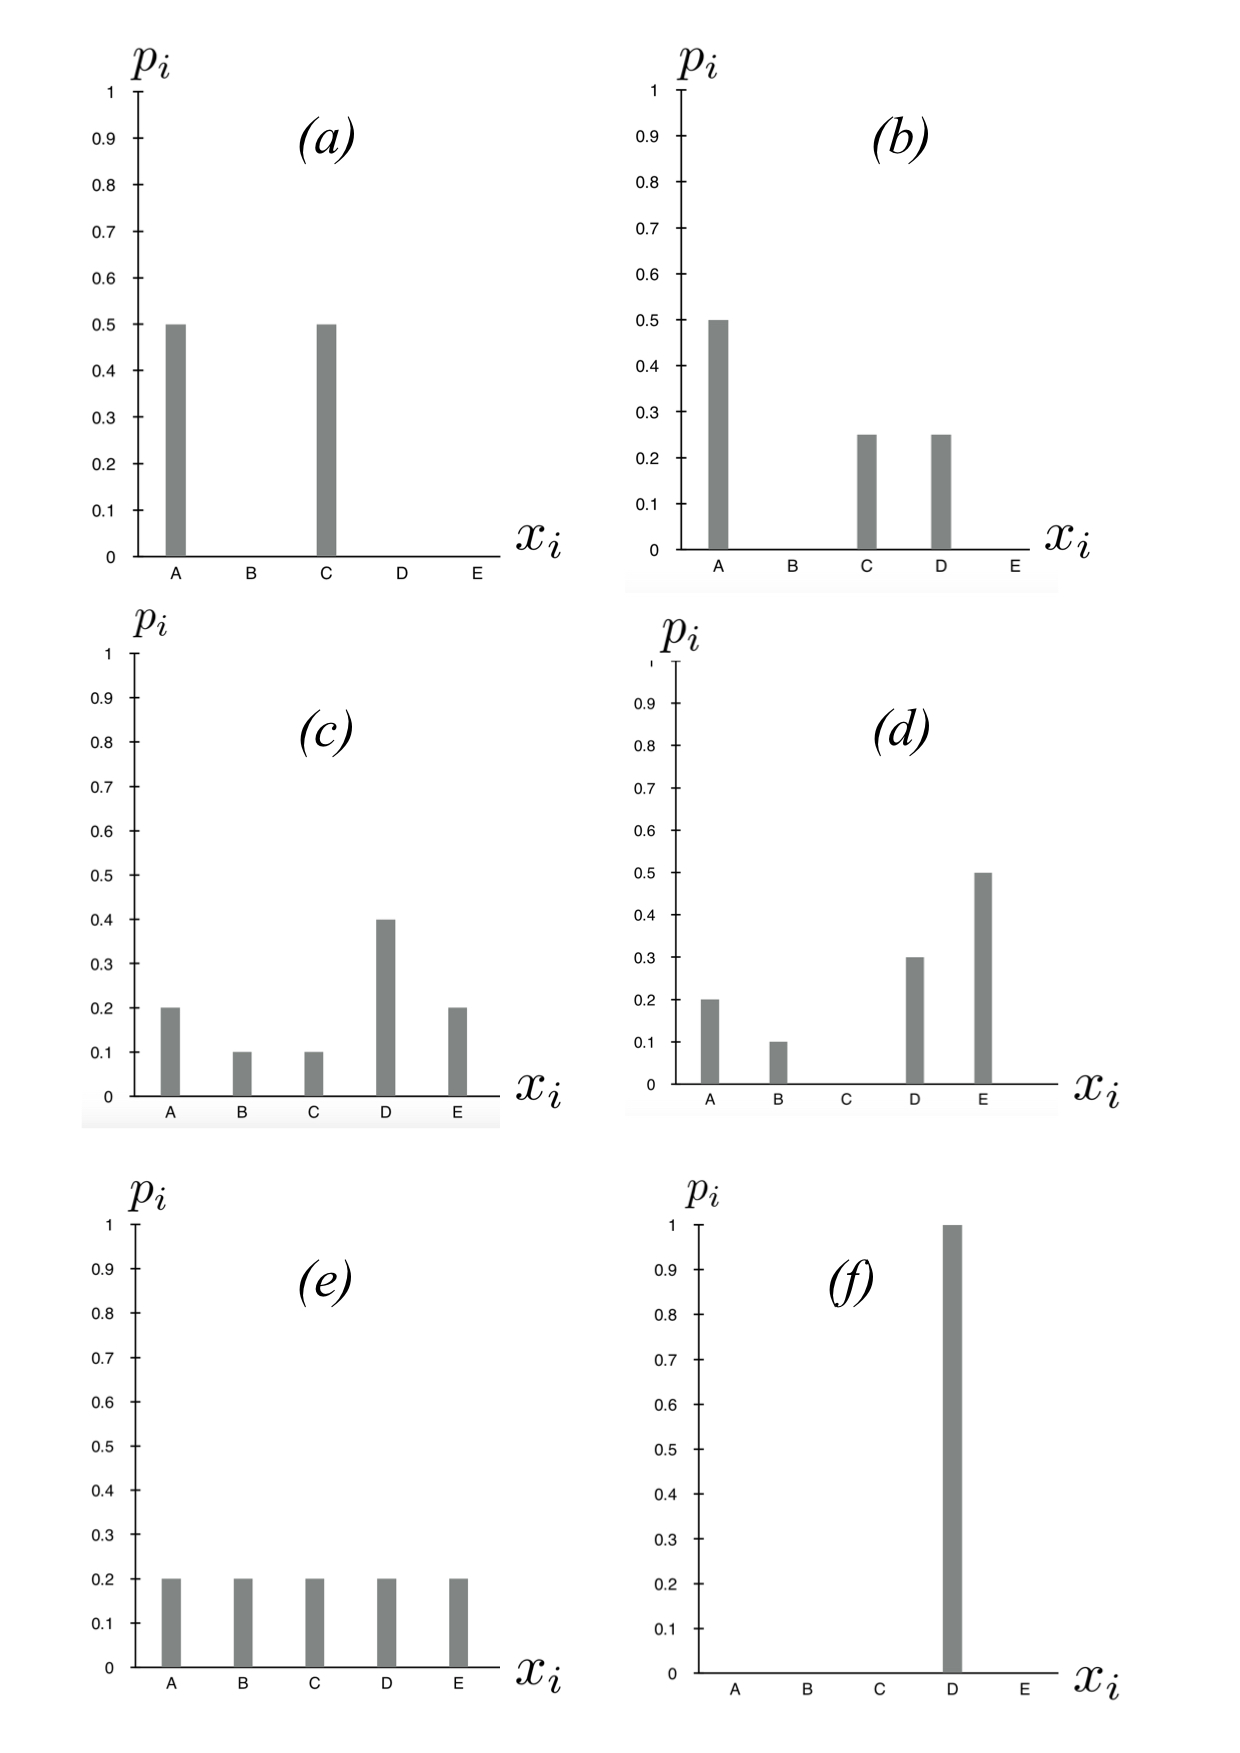
\includegraphics[width = 11 cm, height = 13cm ]{Numbers}%15cm and 20cm
\end{center}
\begin{center}
Figure 2.1 : Some discrete probability distributions\\
\end{center}

%%%gRAPHIC END

Let us calculate the uncertainty associated with each distribution, by arbitrarily taking $k= 1$. We have,\\
 \boxed{\bm{\delta(a)} = \ln2 = \bm{0.69}} 
 \boxed{\bm{\delta(b)} = \frac{3}{2}\ln2 = \bm{1.04}}
 \boxed{\bm{\delta(c)} = \ln5 - \frac{1}{5}\ln2 = \bm{1.47}}
\boxed{\bm{\delta(d)} = \bm{1.26} }
\boxed{ \bm{\delta(e)} = \ln5 = \bm{1.61}} 
\boxed{\bm{\delta(f)} = \bm{0} }

A few observation based on this are:
\begin{enumerate}
\item A distribution like (f) which has a peak at one particular state, has zero uncertainty. That means, it is possible to make a perfect prediction.
\item Distribution (b) has greater uncertainty than (a), which can be interpreted as follows: The system can exist in more states in case (b), therefore, we have less certainty about which state the system is in. 
\item Comparison of states (b), (c) and (d) reveal that uncertainty increases monotonically with the number of states occupied( i.e number of states with non-zero probability of occupation)
\item Comparison of system (c) and (e) reveals that uncertainty is greater when the probabilities are evenly distributed, because in case (c) we can still make some rough guess that the state D is more likely than state B or C, and this information gives us more 'certainty'
\end{enumerate}

Based on these observations regarding the uncertainty function, we come up with the following strategy for optimal prediction:
\begin{mdframed}[style=exercise]
\textbf{Strategy for Optimal Prediction}
 \\* In case of an unknown probability distribution, about which we are to make a prediction, the optimal prediction would be one that maximises the uncertainty.
 \end{mdframed}
 
It is fair, natural and reasonable to propose that the system would be in a 'highly uncertain' distribution, since we actually do not know what the distribution is. This Strategy for Optimal Prediction is often called \textbf{The Axiom of Statistical Mechanics}, and the reader is suggested to convince him/herself of its scientific validity and logical reasonability.\\

Claude Shannon, who fathered 'Information Theory' in the 1940s, used the term \emph{'disorder'} for the same quantity that we have defined as 'uncertainty'. It is indeed true, that the properties of 'uncertainty' are exactly the same as those of 'disorder', and the reader is suggested to pause and ponder over the same, by looking at Figure 2.1.\\

Distribution (f) is the most ordered, whereas distribution (c) is more disordered than distribution (d). However, the term 'uncertainty' keeps the term closely tied to its predictive nature of the problem that we are dealing with here. Nevertheless, we shall henceforth use the terms 'uncertainty' and 'disorder' interchangeably.\\

Thus, taking this strategy to real, physical models, we have the following algorithm: given a system, we write down the constraints, and express the uncertainty as a function of the probabilities of the states. We then \emph{maximise} the uncertainty(or disorder), given the constraints. We accept(according to the axiom of statistical mechanics) that the distribution thus obtained is the most reasonable one that we can predict for it to adopt.\\

However, this algorithm seems uncannily similar to The Entropy Maximum Postulate. In both approaches (phenomenological and statistical), we are maximising a certain quantity associated with a system. Are the entropy of a system and the uncertainty(disorder) related? The answer is that we \emph{can choose to relate} the two approaches. \\

The fact of the matter is, that we can build all of statistical mechanical theory by taking $k$ to be any real constant. Subsequently, all thermodynamic quantities can be defined from scratch using statistical mechanics, but this a cumbersome process. Instead, we make that the clever observation that for any $k$, the disorder(or uncertainty) satisfies the phenomenological postulates of thermodynamics, i.e the disorder is a valid candidate as the possible 'entropy' function associated with a system.\\

It can be shown that assigning $k = k_B$ in Definition 2.2, ensures that the uncertainty is \emph{exactly} equal to the entropy defined phenomenologically, and that this choice of constant leads to perfect completeness as far as the units and values of all thermodynamic quantities are concerned.
\\

 The following definition, thus, is the unifying principle in thermodynamics and thermostatistics, and its validity, importance and relevance can not be overstated (More discussions on the same will be made in Chapter 3) :

\begin{mdframed}[style=exercise]
\textbf{Definition 2.3}
 \\* The Entropy $(S)$ associated with a discrete probability distribution consisting of discrete random variables $x_1,x_2,x_3,...,x_n$ with associated probabilities $p_1,p_2,p_3,....,p_n$ is given by
 \[ S = -k_B\sum_{i= 1}^{n}p_i\ln(p_i) \]
 where $k_B$ is the Boltzmann constant (defined in Section 1.4)
 \end{mdframed}
 




\section{The Optimal Prediction}

 \begin{mdframed}[style=exercise]
\textbf{Definition 2.4}
 \\* An isolated system is one that does not interact with the rest of the universe through any mechanism. It follows, that no observer can make any measurement on an isolated system. It is also assumed that the probability distribution of the states of an isolated system does not change with time.
 \end{mdframed}
Let us look at the probability distribution of an isolated system.

\begin{mdframed}[style=exercise]
\textbf{Example 2.1}
 \\* Consider a system in which some constraint is released, and it is subsequently isolated. The system can now exist in $n$ states $x_1,....,x_n$. Find the probability distribution of the system.
 \end{mdframed}
 \textbf{Solution} We are not given any constraints, and we are to make a prediction regarding the future state of the system. We follow the axiom of statistical mechanics, and make the most 'uncertain' prediction possible, i.e\\
 we maximise the uncertainty
 \[ \delta = -k\sum_{i= 1}^{n}p_i\ln(p_i)\]
 with
 \[\sum_{i =1}^{n}p_i = 1 \]
 For this maximisation, we use the Lagrange Multiplier Method. We let $\nabla \delta(p_1,...p_n) = \lambda \Bigg[\nabla \Big(\big(\sum_{i =1}^{n}p_i \big)- 1\Big)\Bigg]$\\
 Solving these n equations simultaneously gives us $-k(1 + \ln(p_i) )= \lambda$; i.e 
 \[p_1 = p_2 = p_3 = ... = p_n = e^{-(\frac{\lambda}{k} + 1}) \]
 Using $\sum_{i =1}^{n}p_i = 1$, we obtain 
  \[p_1 = p_2 = p_3 = ... = p_n = \frac{1}{n} \] \\
  
This result might seem too good to be true, but it is not. We simply make the \emph{optimal prediction} by maximising the uncertainty. The point to be noted here is \emph{that there are no constraints.} Then a logical question would be, "when do constraints arise?" \\

Constraints arise when a system is not truly \emph{isolated}, but interacts with the rest of the universe(and most importantly, the observer) through some form of matter or energy. If a system is not isolated, we can exploit its interaction with the rest of the universe to make \emph{some} observation that would give us \emph{some} constraint that would likely shake up the probability distribution. But in case we can't make an observation, the only thing we can do is maximise our uncertainty about the system, which results in each state having equal probability.\\

A gas enclosed in a container is constrained, and we can conclude with confidence that for it $V$ is fixed. Observations made on the container would tell us the energy $(U)$ and mole numbers$(N_1,...,N_R)$ of the components of this system. However, we may come to know that are $n$ valid microstates that produce the same set of macroscopic coordinates. The \emph{new} system consisting of only the microstates is 'isolated', and we have no way of knowing anything about it. What is the probability distribution among these microstates? If we are to predict this distribution, we would follow exactly the same steps as given above, and would be led to conclude that all microstates have equal probabilities.\\

Thus, the power of the result obtained above becomes evident when we start to consider quantum mechanical microstates. We simply maximise our uncertainty about an isolated system, and the optimal prediction that pops out is that the system is equally likely to be in any of the microstates. In this case, the uncertainty, when maximised, becomes $k\ln(n)$, where $n$ is the number of states that can be occupied by an isolated system.\\ \\ 
If we are to use $k = k_B$, we derive a powerful formula for the entropy of an isolated system that can exist in $W$ states. It is known as Boltzmann's Formula:

\begin{center}
\boxed{S = k_B\ln(W)}
\end{center}

Most generally, this formula is applied to systems that are \emph{assumed} to be isolated, like the sub-system comprising of the microstates of a system whose macroscopic coordinates are fixed. In such cases, the number of microstates $W$ is a function of the macroscopic state of the system, i.e $W = W(U,V,N_1,...)$. Using this formulation, we can find the equation of state of an isolated system, and it only involves the counting of the number of states available as a function of the extensive parameters.

 \begin{mdframed}[style=exercise]
\textbf{Example 2.2}
 \\* Consider a system which has the only variable extensive parameter as the energy (i.e $V, N_1,...,N_r$ are fixed and determinate). Some constraint is released so that the (energy)states can take any probability distribution. On multiple observations of different copies of the system, we find that the average total energy of the system is $U$. Find the probability distribution of the states of the system.
 \end{mdframed}
 \textbf{Solution} We say that the system can be in any (macro)state $x_j$ with associated energy $E_j$. The probability of occupation of the $j^{th}$ state is $p_j$. For finding the probability distribution, we maximise the uncertainty
 \[ \delta = -k\sum_{j}^{}p_j\ln(p_j)\]
 subject to 
  \[\sum_{j}^{}p_j = 1 \]
  and
  \[\sum_{j}^{}p_jE_j = U \]
   Using the Lagrange Multiplier Method, we write
  \[  \nabla \Big[-k\sum_{j}^{}p_j\ln(p_j)\Big] = \lambda_1\nabla\Big[\sum_{j}^{}p_j - 1\big] +\lambda_2\nabla\Big[\sum_{j}^{}p_jE_j - U \Big]\]
 This gives us 
 \[\ln(p_j) + 1 + \lambda_1 + \lambda_2E_j  = 0 \]
 or
 \[ p_j = e^{-(1 + \lambda_1 + \lambda_2E_j)}\]
 where $\lambda_1$ and $\lambda_2$ are determined from the equations:
 
 \[ e^{-(1 + \lambda_1)} \sum_{j}^{}e^{-\lambda_2E_j} = 1
 \hspace{0.5cm} and \hspace{0.5cm}
 e^{-(1 + \lambda_1)} \sum_{j}^{}E_je^{-\lambda_2E_j} = U\]
 Writing $\lambda_1 = \beta$ and $\sum_{j}^{}e^{-\beta E_j} = Z$ allows us to write $p_j$ compactly as
  \[ p_j = \frac{e^{-\beta E_j}}{Z}\]
 

 \begin{mdframed}[style=exercise]
\textbf{Example 2.3}
 \\* Consider a system which has the only variable extensive parameters as the energy and the number of moles of the single component that the system is composed of. Some constraint is released so that the states can take any probability distribution. On multiple observations of different copies of the system, we find that the average total energy of the system is $U$, and the number of moles observed is $N^0$ . Find the probability distribution of the states of the system.
 \end{mdframed}
 \textbf{Solution} We proceed exactly as in Example 2.2, maximising the uncertainty 
 \[ \delta = -k\sum_{j}^{}p_j\ln(p_j)\]
 subject to 
  \[\sum_{j}^{}p_j = 1\hspace{0.2cm};\hspace{0.2cm} \sum_{j}^{}p_jE_j = U\hspace{0.2cm}; \hspace{0.2cm} \sum_{j}^{}p_jN_j = N^0\]
  We again use Lagrange Multipliers, giving us
   \[ p_j = e^{-(1 + \lambda_1 + \lambda_2E_j + \lambda_3N_j)}\]
where $\lambda_1,\lambda_2,\lambda_3$, can be eliminated amongst the three constraints.


\section{Boltzmann's Formula}
We shall extensively use Boltzmann's Formula, derived quite accidentally in Example 2.1. It not only connects the Entropy to the disorder and uncertainty, but also allows us to easily calculate the equation of state for an \emph{approximately} isolated system.\\

What is the use of this formula in a system that is not isolated? The powerful trick, is to consider this system in contact with another system, such that this composite system may be approximated to be isolated.\\

Reservoirs are axiomatically taken to be isolated. It is possible to assume a model in which a system is in contact with a reservoir. This composite system of (system + reservoir) can then be assumed to be isolated, and Boltzmann's Formula can be applied.

 \begin{mdframed}[style=exercise]
\textbf{Example 2.4}
 \\* Consider a system in contact with a heat reservoir at Temperature $T$, and having all other parameters except the Energy fixed. Find the probability distribution of the (energy)states.
 \end{mdframed}
\textbf{Solution} 
We assume that the (subsystem + reservoir) composition is isolated.\\

Let the number of states available for occupation by the subsystem, reservoir and composition(of subsystem + reservoir) be given (as a function of the energy $E$) by 
$W_{sys}(E), W_{res}(E)$ and $W_{tot}(E)$ respectively. At any instant, we have
 $E_{sys} + E_{res} = E_{tot}$, where $E_{tot}$ is a large, arbitrary energy that we assume the net composition to be having.\\

Now, $W_{res}$ is completely independent of what (energy)state the subsystem is in, and depends only on $E_{res}$. Therefore, the number of (energy)states of the whole system for which the subsystem is in a desired state $j$, having energy $E_j$ is simply given by

\[W_{sys}(E_j) = W_{res}(E_{res}) = W_{res}(E_{tot} - E_j) \]

 This gives us 

\[p_j =  \frac{W_{sys}(E_j)}{W_{tot}(E_{tot})} = \frac{W_{res}(E_{tot} - E_j)}{W_{tot}(E_{tot})}  \] \\ \\

Since the reservoir and the total composition are both isolated, we have definite entropies for them, given by Boltzmann's Formula, which lead to

\[p_j = \frac{  exp[\frac{S_{res}{(E_{tot} - E_j)}}{k_B}]  }{  exp[\frac{S_{tot}{(E_{tot})}}{k_B}]  } \]

Let $U$ be the average value of the energy of the system(whose value we don't know of, yet). We write 
\[  S_{tot}(E_{tot}) =   S_{sys}(U) + S_{res}(E_{tot} - U)\]
and
\[ S_{res}(E_{tot} - E_j) =  S_{res}(E_{tot} - U + U - E_j) = S_{res}(E_{tot} - U) + \frac{(U - E_j)}{T}  \]
which allows to recast $p_j$ in the form

\[p_j = e^{ \frac{U-TS(U)}{k_BT}  }   e^{    -\frac{E_j}{k_BT}   } \]

We let $\frac{1}{k_BT} = \beta$, which gives us 

\[p_j = e^{ \beta{\big(U-TS(U)\big)}  }   e^{    -\beta{E_j}   } \]

Noting that $U-TS(U) = F$, the Helmholtz Free Energy of the whole system, we obtain 

\[ \sum_{j}^{}e^{-\beta E_j} = e^{-\beta F} \]

We call $e^{-\beta F} = Z$, or 'The Partition Sum'. This gives us 

  \[ p_j = \frac{e^{-\beta E_j}}{Z}\]
  
 This result is exactly the same as that obtained in Example 2.2. The difference in the two cases is that in Example 2.2, the average (expected) energy of the system was fixed, and we calculated the two Lagrange Multipliers by simply maximising the disorder, i.e we calculated two unknowns from one known parameter. \\
 
Here, we do the same. it is just that the known parameter is different. We assume a system in contact with a heat reservoir at temeperature $T$ and we know beforehand that
 $\beta = \frac{1}{k_BT}$. The energy of the system and the entropy are unknowns, which we calculate using
 
 \[ U = \sum_{j}^{}p_jE_j\]
 
 and
 
 \[ S = \frac{U}{T} + \frac{F}{T} = k_B\beta\sum_{j}^{}p_jE_j + k_B\ln Z\]
 


This is probably one of \emph{the most} important derivations in Statistical Mechanics, and the model developed here by assuming a system in thermal contact with a heat reservoir, is called \textbf{The Canonical Formulation}, which is summarised below in five equations: \\ 
\begin{mdframed}[style=exercise]
\[\frac{1}{k_BT} = \beta
\hspace{0.3cm};\hspace{0.3cm} 
\sum_{j}^{}e^{-\beta E_j} =  Z      
\hspace{0.3cm};\hspace{0.3cm}
 p_j = \frac{e^{-\beta E_j}}{Z}
\hspace{0.3cm};\hspace{0.3cm}
U = \sum_{j}^{}p_jE_j
\hspace{0.3cm};\hspace{0.3cm}
S = k_B\beta\sum_{j}^{}p_jE_j + k_B\ln Z
\]
\end{mdframed}
In hindsight, we can conclude with confidence that one of the Lagrange multipliers obtained in Example 2.2, did indeed correspond to the temperature, i.e we could have obtained $T$ for that system as 
$T = \frac{1}{k_B\beta}$. The Canonical Formalism and Example 2.2 are two sides of the same coin, and the reader is suggested to ponder over the subtle difference between the two.

 \begin{mdframed}[style=exercise]
\textbf{Example 2.5}
 \\* 
 Consider a system in contact with a heat reservoir at Temperature $T$, and a particle reservoir with Chemical Potential $\mu$. Find the probability distribution of the states.
 \end{mdframed}
\textbf{Solution} We proceed \emph{exactly} as in Example 2.4, assuming the composition of (subsystem + reservoirs) to be isolated. We obtain

\[p_j =  \frac{W_{sys}(E_j, N_j)}{W_{tot}(E_{tot}, N_{tot})} = \frac{W_{res}(E_{tot} - E_j, N_{tot} - N_j)}{W_{tot}(E_{tot}, N_{tot})}  \]

Expressing $W$ in terms of entropy, we have

\[p_j =   exp[\frac{S_{res}{(E_{tot} - E_j, N_{tot} - N_j)}}{k_B} - \frac{S_{tot}{(E_{tot}, N_{tot})}}{k_B}]   \]

Proceeding as in the previous example, we obtain


\[p_j = e^{ \beta \Psi  }   e^{    -\beta{(E_j - \mu N_j)}   } \]

By suitably renaming the terms, we obtain what is known as \textbf{The Grand Canonical Formulation}, summarised below:
\begin{mdframed}[style=exercise]
\[\frac{1}{k_BT} = \beta
\hspace{0.3cm};\hspace{0.3cm} 
e^{-\beta \Psi} = \sum_{j}^{}e^{-\beta (E_j - \mu N_j)} =  Z_0      
\hspace{0.3cm};\hspace{0.3cm}
 p_j = \frac{e^{-\beta (E_j - \mu N_j)}}{Z_0}
\hspace{0.1cm}; 
\]
\[U = \sum_{j}^{}p_jE_j
\hspace{0.3cm};\hspace{0.3cm}
N = \sum_{j}^{}p_jN_j
\hspace{0.3cm};\hspace{0.3cm}
\Psi = U - TS(U,N) - \mu N \]
\end{mdframed}

These equations may seem unpalatable at first glance. However, considering the mathematical weight that most Statistical Mechanical derivations carry(especially those that we shall encounter in Section 2.5), whatever we have seen till now has been pretty light. Here's a quote to cheer the reader on, for the next section: \\
\begin{center}
\emph{" If you are out to describe the truth,}\\
\emph{leave elegance to the tailor"}\\
\emph{\hspace{5cm}-Ludwig Boltzmann}\\
\end{center}

\section{Describing the truth}

In this section, we shall be using our statistical mechanical repertoire to solve real, physical problems, by suggesting models for each system. 

\subsection{The Einstein Crystal}
We attempt to come up with the fundamental equation for a non-metallic crystalline solid. Albert Einstein came up with the (simplistic) model that individual atoms in a crystal are harmonically bound to their neighbouring atoms. Accordingly, the vibrational modes are strongly coupled. \\

Wave mechanics tells us that there will be $3N$ collective normal modes, where $N$ is the number of atoms we are considering in the crystal. The frequencies of vibration are quantised(since the model corresponds to a quantum harmonic oscillator). We choose the zero of energy such that the frequencies are of the form $\omega = n\hbar\omega_0$, where $n$ is a whole number, that ranges from 0 to $ \infty $.\\

Consider \emph{one} atom in this crystal as a \emph{subsystem}. This subsystem has energies $E_1, E_2, E_3, E_4...$ given by $0, \hbar\omega_0, 2\hbar\omega_0, 3\hbar\omega_0,...$\\ \\ \\ \\ \\

For this one subsystem, we calculate $Z_{sub}$ as given by

\[ Z_{sub} = \sum_{n}^{}e^{-\beta E_n} =  \sum_{n = 0}^{\infty}e^{-\beta n\hbar\omega_0} \] 

where $\beta = \frac{1}{k_BT} $, and $T$ is the temperature of the crystal. We sum up the infinite geometric progression to obtain 

\[ Z_{sub} = \frac{1}{1 - e^{-\beta\hbar\omega_0}}\]

The whole crystal can thus be modelled as a composite system of $N$ such \emph{subsystems}, with the total energy of the crystal being equal to the the sums of the energies of the individual subsystems. This gives us

\[Z_{tot} = \sum_{subsystems}^{}e^{-\beta({E_{sub1} + E_{sub2}+ E_{sub3}.......) }} 
= \sum_{subsystems}^{}e^{-\beta E_{sub1}}e^{-\beta E_{sub2}}e^{-\beta E_{sub3}}....\]
\[= \sum_{n}^{}e^{-\beta E_{sub1}} \sum_{n'}^{}e^{-\beta E_{sub2}} \sum_{n''}^{}e^{-\beta E_{sub3}}....
= Z_{sub1}Z_{sub2}Z_{sub3}.... = \prod_{subsystems}^{}Z_{sub}\]

The assumption made by Einstein was that every atom would have the same frequency of vibration. For the crystal with $N$ atoms (and 3N modes of vibration), this gives us:

\[Z_{tot} = \Big(Z_{sub}\Big)^{3N} = \Big(\frac{1}{1 - e^{-\beta\hbar\omega_0}}\Big)^{3N}\]

Now that we have $Z$ for the crystal, we find the equation of state for the system

\[ F =  -\frac{1}{\beta} \ln{(Z_{sub})^{3N}} = 3Nk_BT\ln{(1 - e^{-\beta\hbar\omega_0 })} \]

and use $U = \sum_{n =0}^{\infty}\frac{E_ne^{-\beta E_n}}{Z}$ to find 

\begin{center}
\boxed{U = \frac{3N\hbar\omega_0}{1 - e^{-\frac{\hbar\omega_0}{k_BT}}}}
\end{center}

We find that the heat capacity of this crystal $(c_v = \frac{\partial U}{\partial T})$ tends to zero as $T\rightarrow 0$ and $c_v\rightarrow 3R$ as $T\rightarrow \infty$. This experimentally validates the model.


\subsection{The Particle In a Box}
The main aim of this section is to motivate the existence of 'the density of states' function.\\ \\
We know that for a 'particle'(wavicle, if you prefer), in a 3-D box, we have its wavelength quantized, i.e

\[ \textbf{k} = \frac{\pi}{L}(n_x \hat{\textbf{ x }} + n_y\hat{\textbf{ y }}  + n_z \hat{\textbf{ z }}  ) \]
where $n_1,n_2,n_3$ are integers. The generality of the above statement is extremely powerful, as it holds for any entity that is trapped in a box of dimensions $L \times L \times L $. We write $L = V^{\frac{1}{3}}$, $V$ being the volume of the box.\\

We ask, what is the number of states that lie in the interval $(k, k + dk)$? \\

The number of states that a system can take, given a particular $k$, is the number of positive integers for which

\[ (n_x^2 + n_y^2 +n_z^2 )^\frac{1}{2} \leq \frac{V^{\frac{1}{3}} k }{\pi}\]

We can interpret $(n_x^2 + n_y^2 +n_z^2 )^\frac{1}{2} $ as the radius in an abstract space where the coordinate axes are $n_x,n_y,n_z$. \\

The number of states available to a system, given a $k$, is equal to the number lattice points in the first octant, with radii less than 
$\frac{V^{\frac{1}{3}} k }{\pi} $. This leads us to conclude that the number of states available in the interval $(k, k + dk)$, is equal to the the number of lattice points in the volume enclosed by the shell in the first octant having radius $\frac{V^{\frac{1}{3}} k }{\pi} $.\\

In mathematics, this is known as the 'Gauss Circle Problem'. Bounds on the solution to this problem allow us to approximate that the number of lattice points whose distance from the origin is less than a particular value $R$, is simply equal to the volume of the sphere in the first octant having radius $R$. Hence, we find the volume of the shell between $R$ and $R + dR$ as $\frac{1}{8}(4\pi R^2)dR$. Putting $R = \frac{V^{\frac{1}{3}} k }{\pi} $, we obtain the number of states between $k$ and $k+dk$  (called $g(k)dk$ ) as

\begin{center}
\boxed{ g(k)dk = \frac{V}{2\pi^2}k^2dk}
\end{center}

Here, $g(k)dk$ is called \textbf{The Density of States Function}. It is used when the energy is a function of k, and the difference between consecutive energy states is very less, which leads to 'blurring' (especially in the classical limit) of the discrete states. In this case, we do not calculate energies by summing up discrete states, but do so by \emph{integrating} as follows:

\[  \sum_{j}^{}E_je^{-\beta E_j} \hspace{0.5cm} \longrightarrow \hspace{0.5cm} \int_{k}^{} E(k)e^{-\beta E(k)} g(k)dk \]

\subsection{Electromagnetic Radiation}
We consider electromagnetic radiation that is contained within a closed vessel with perfectly conducting walls. The energy may be considered to be residing in the resonant electromagnetic modes of the cavity, or in the photons occupying the cavity. Both the models are mathematically equivalent, and we shall be considering the photons occupying the cavity.\\

For photons, we have $E = pc$ and $p = \hbar k$. Proceeding as in Section 2.5.1, we obtain 

\[ F =  k_BT\sum_{all \hspace{0.1cm} modes}^{}\ln{(1 - e^{-\beta \hbar kc})} \]

This sum is calculated by using the density of states function, as defined in Section 2.5.2:

\[ F =  k_BT\int_{0}^{\infty}\ln{(1 - e^{-\beta \hbar kc})g(k)dk} = k_BT\int_{0}^{\infty}\ln{(1 - e^{-\beta \hbar kc})\frac{V}{2\pi^2}k^2dk}  \]

For the Canonical Formalism, we have $U = \sum_{j}^{} \frac{e^{-\beta E_j}E_j}{\sum_{j}^{} e^{-\beta E_j}} $ which gives us \[ U = - \Big( \frac{d}{d\beta} \Big)\ln Z = \frac{d}{d\beta} \Big( \beta F \Big) \] \\

Using, this, we calculate $U$ from $F$, leading to

\[ U = \frac{Vc\hbar}{\pi^2} \int_{0}^{\infty}\frac{e^{-\beta \hbar c k }k^3dk}{1 - e^{-\beta \hbar ck}}  \]

On evaluating this integral, we obtain what is known as \textbf{The Stefan-Boltzmann Law}:\\

\begin{center}
\boxed{U = \frac{\pi^2k_B^4}{15\hbar^3c^3}VT^4}
\end{center}

\subsection{The Hydrogen Atom}
For a one-electron Hydrogen Atom, we can write the net wavefunction as a product of the nuclear wavefunction and the electronic wavefunction, i.e

\[ \Psi = \Psi_{nuclear}\Psi_{electronic}\]

$\Psi_{nuclear}$ is the same as that of a free particle. Solutions to the Schrödinger equation for the electronic part $\hat{H}_e\psi(r,\theta,\phi) = E\psi(r,\theta,\phi)$ (where 
$\hat{H}_e$ is the electronic Hamiltonian), reveal that $\psi(r,\theta,\phi)$ is of the form

\[ \psi(r,\theta,\phi) = R_{n,l}(r) \times Y_{l}^m(\theta,\phi) \]

where $R_{n,l}(r)$ is called the 'radial part' of the function and $Y_{l}^m(\theta,\phi)$ is called the 'angular part' of the electronic wavefunction. Putting in specific values of quantum numbers $n,l$ and $m$ give us different orbitals. If we are to define an orbital by the ordered triplet $(n,l,m)$ then each orbital is a 'state' that the electron can be in.\\

We shall depict orbitals using the notation $\psi_{(n,l,m)}$. This notation is often expanded: $\psi_{(1,0,0)}$ is called the $1s$ orbital, $\psi_{(2,0,0)}$ is called the $2s$ orbital, and so on. This notation allows to write the net electronic wavefunction as a superposition of the different orbitals as follows:

\[ \Psi_{electronic} =  c_{(1,0,0)}\psi_{(1,0,0)} + c_{(2,0,0)}\psi_{(1,0,0)} + c_{(2,1,0)}\psi_{(1,0,0)} + .....\] 

or

\[ \Psi_{electronic} =  c_{1s}\psi_{1s} + c_{2s}\psi_{2s} + c_{2p_z}\psi_{2p_z} + .....\] 

The only problem is that the values of the coefficents $ c_{1s}, c_{2s},c_{2p_z},...$  are unknown, and can't be determined quantum mechanically. However, this task is right up the statistical physicist's alley.\\

The predictive nature of statistical mechanics, allows us to easily calculate 'the probability of occupation' of an orbital. For a given state $\psi_{(n,l,m)}$, the energy is given by 

\[  E_{(n,l,m)} = -\frac{A}{n^2}  \]

where $A = 13.6$ eV. Consider a gas of hydrogen molecules at Temperature $T$. The Canonical Formulation gives us

\[[c_{(n,l,m)}]^2 = p_{(n,l,m)} = \frac{e^{-\beta E_{(n,l,m)}}}{Z} \]

Now, each energy level characterised by $'n'$ is degenerate. The degenerate orbitals have equal probabilities of occupation. For calculating $Z$, we must introduce a degeneracy factor $g_n$ for every energy level, which in this case is given by
\[g_n = 2n^2 \]

 This gives us

\[ p_n = \frac{g_ne^{ -\beta E_n } }{ \sum_{n = 1}^{\infty}g_ne^{ -\beta E_n}  } = \frac{n^2e^{ \frac{A}{n^2k_BT} } }{ \sum_{n = 1}^{\infty}n^2e^{ \frac{A}{n^2k_BT} } }  \]

Here we have characterised every energy level using $n$ alone. In this notation, we would obtain \[ p_{2s} = p_{2p_x} = p_{2p_y} = p_{2p_z} = \frac{p_{2}}{g_2}\]

Using this formula, we can easily calculate the coefficients required in the electronic wavefunction. 


The important takeaway from this derivation is that 
\begin{enumerate}
\item The probability of occupation of the ground state, i.e $(n =1)$ is the highest at a given temperature. In fact, the ration of $c_{2}$ to $c_{1}$ at $T$ = 300 K is $4e^{-395} \approx 0$. This also confirms our 'classical' belief that an undisturbed hydrogen atom will most likely be in the ground state. 
\item At higher Temperatures, the probability of occupation of higher energy levels increases. At 20,000 K, the ratio of $c_{2}$ to $c_{1}$ is approximately 0.01
\end{enumerate}

These facts leads to extremely important simplifications, that validate Classical Chemistry. Also, the model developed here neatly explains the emission spectra of hydrogen, and forms the basis for a wide range of spectroscopic study.\\

What if we are to have multiple electrons in a hydrogen atom? In that case we can't use this model because the electronic wavefunction would be different, $E_n$ would be different and we would have to use approximations. If we know $E_n$, we can make statistical predictions.\\

This leads us to an interesting, and far more general question: What if we consider a system consisting of discrete, known, energy levels, in which a total number of 'particles' are to be distributed? How would the distribution look?\\

The answer is that, it depends on the type of 'particle'.\\

In quantum mechanics, every 'particle' is classified into either one of, two categories: it is either a \textbf{Fermion} or a \textbf{Boson}. As far as this text is concerned, we shall not define what either of them are, but shall only look at some of their properties:

\begin{enumerate}
\item Fermions are the quantum mechanical analogues of classical, material 'particles'. Electrons, protons, and neutrons are some examples fermions. A defining characteristic of fermions is that the net wavefunction is antisymmetric under interchange of any two fermions. This leads to an immediate consequence: \emph{"No two fermions can occupy the same orbital."} Also, both fermions and bosons have a classically-indescribable multi-valuedness, called 'spin'. Fermions have spin that are odd-integral multiples of $\frac{1}{2}$
\item Bosons are the quantum mechanical analogues of classical 'waves'. Just like waves, bosons can be superposed, and multiple bosons can occupy the same orbital. Bosons have a spin that is an even-integral multiple of $\frac{1}{2}$. Photons are an example of bosonic particles. 
\end{enumerate}

On the basis of these few general properties, we shall attempt to develop models for the statistical distributions of fermions and bosons in the coming sections.

\subsection{Fermi-Dirac Statistics}
We shall consider a very simple, yet general, fermionic system in this section. It can easily be expanded to cover the broadest of cases.\\

For brevity, we shall consider this system to consist of two discrete and fixed energy levels, having energies $\epsilon_1$ and 
$\epsilon_2$. The whole system is in equilibrium with a thermal reservoir at Temperature $T$. It is also in equilibrium with a half-spin-fermion reservoir having Chemical Potential $\mu$.\\

The system conditions call for the usage of the Grand Canonical Formalism. To find the probability of the system being in on state, we need to find the Grand Partition Sum $Z_0$.\\

Just as in the Einstein Crystal, we shall consider the whole system to be made of smaller, independent subsystems whose energies add up, such that 

\[Z_{0} = \prod_{subsystems}^{}Z_{sub}\]

What shall we choose as our subsystems? There is one particular choice of a set of subsystems that leads to profound consequences in the development of this theory, and we shall adopt this choice: We consider every 'orbital' to be a subsystem.\\

In our particular example, an orbital is identified by two constants: $n$ and $m_s$: $n$ is associated with the energy level and can take two values: 1 or 2, while $m_s$ is associated with the spin and can take values $+\frac{1}{2}$ or $-\frac{1}{2}$\\

This choice quickly tells us that our system is composed of four subsystems, whose characteristic 'quantum numbers' are listed here: $(1,+\frac{1}{2}), (1,-\frac{1}{2}), (2,+\frac{1}{2})$ and $(2,-\frac{1}{2})$. The benefits of choosing these four systems are illustrated below:

\begin{enumerate}
\item Each subsystem is isolated, because it is only in contact with reservoirs. 
\item Each of these subsystems can be filled by atmost one fermion. If there were more than one fermion in one subsystem, it would violate the antisymmetry principle. 
\item Our job of dealing with the subsystems is thus simplified to a marvellous extent. Each of these subsystems can be \emph{filled independently}, and can be in either of the two states: filled or empty. The filling of one subsystem does not affect the filling of any other subsystem in any way, and is quantum mechanically sound.
\item We can choose a convention of labelling our subsystems. We call the subsystems $(1,+\frac{1}{2})$, $(1,-\frac{1}{2}), (2,+\frac{1}{2}), (2,-\frac{1}{2})$ as A,B,C and D respectively. We represent the state of the whole system as a binary number $abcd$ where each of $a,b,c$ and $d$ can be either 0 or 1. $a$ being 1 corresponds to the subsystem A being filled, and $a$ being 0 corresponds to A being empty. Our convention applies similarly to $b,c,d$. We shall refer to any four-digit binary number that represents the state of this system as ' a configuration' of the system. Thus there are 16 configurations that our system can be in.
\item The energies of these subsystems add up, and hence we can obtain the Grand Partition Sum by simply multiplying the partition sums of each of these subsystems.
\end{enumerate}

The partition sum for a subsystem with quantum numbers $(m,n)$ in this case is given by

\[z_{(n,m)} =  \sum_{N_j =0}^{1}e^{-\beta(E_n-\mu N_j)} = 1 + e^{-\beta(E_n-\mu)}\]

Using this, we obtain

\[Z_{0} = z_Az_Bz_Cz_D = (1 + e^{-\beta(\epsilon_1-\mu)})^2(1 + e^{-\beta(\epsilon_2-\mu)})^2\]

For an arbitrary configuration $abcd$, we now have:

\[ p_{abcd} = \frac{e^{-\beta (E_{abcd} - \mu N_{abcd})}}{Z_0}\]

We can find the total energy of the configuration using

\[ U = \sum_{configurations}^{}p_{abcd}E_{abcd}\]

and the total number of fermions present in the system by

\[ N_t = \sum_{configurations}^{}p_{abcd}N_{abcd}\]

This last equation is of particular interest. In general, it is difficult to physically create a particle reservoir, and it is often easier for a system to have the total number of particles $N_t$ fixed. In this case, $\mu$ becomes a variable, that can be easily determined using the last equation. The RHS is a function of $\mu$, and having knowledge about $N_t$ allows us to numerically calculate a value for $\mu$ for a given system.\\

Thus, in general, we start with two known parameters about a fermionic system: its temperature, and the total number of particles. We then use the equations above to find the the $\mu$ associated with the system, and subsequently find its partition sum, probability of a particular configuration, total energy, and equation of state using $-\beta\Psi = \ln Z_0$\\

In essence, we are done with our system. We broke it up into individual subsystems that were like 'rooms', that could either be filled or empty. Doing this, we could find the equation of state, and the probabilities of different configurations that the system could be in. This is the general algorithm for solving any fermionic system.\\

The analysis of fermionic systems can end here. However, a few clever manipulations can allow us to extract far more from this method.\\

Let us for a moment, consider the rather arbitrary question, "If we consider each 'orbital', or 'subsystem' to be a \emph{system} in itself(in contact with thermal and particle reservoirs), what is the probability of this \emph{system} being in a particular state?"\\

This 'orbital' can be in either of the two states: filled or unfilled. This gives us

\[p(filled)_{(n,m)} = \frac{e^{-\beta(E_{(n,m)} - \mu)}}{z_{(n,m)}} \hspace{0.5cm}and\hspace{0.5cm}
p(unfilled) _{(n,m)}= \frac{1}{z_{(n,m)}}\]

We introduce some new notation here. We call $p(filled)_{(n,m)}$ as $f_{nm}$ and $p(unfilled) _{(n,m)} $ as $f'_{(n,m)}$. Using $z_{(n,m)} =  1 + e^{-\beta(E_n-\mu)} $, we obtain

\begin{center}
\boxed{f_{nm} = \frac{1}{e^{\beta(E_{n} - \mu)}+ 1} }
\end{center}

This is a very powerful formula that is true in general for any fermionic system whose energy levels are characterised by $n$. With reference to our specific two-energy-level system, $f_{nm}$ takes the form

\[ f_A = f_B = \frac{1}{e^{\beta(\epsilon_{1} - \mu)}+ 1}\hspace{0.5cm};\hspace{0.5cm} 
f_C = f_D = \frac{1}{e^{\beta(\epsilon_{2} - \mu)}+ 1}\]

Let us consider, in our labelled two-energy-level system, the probability of the configurations (1000), (0100), (1010), (0111). It is easy to see that

\[  p_{(1000)} = f_Af'_Bf'_Cf'_D \hspace{0.1cm} ; \hspace{0.1cm} p_{(0100)} = f'_Af_Bf'_Cf'_D  
 \hspace{0.1cm} ; \hspace{0.1cm} p_{(1010)} = f_Af'_Bf_Cf'_D  \hspace{0.1cm} ; \hspace{0.1cm} p_{(0111)} = f'_Af_Bf_Cf_D \]

Such a relationship exists for any configuration of the composite system, and is true for all general, fermionic systems. Thus, we see that $f_{nm}$ is a simple function that is easy to calculate for any 'orbital' or 'room', and allows us to calculate the probabilities of larger configurations very neatly. \\

However, there are two \emph{very} surprising results related to $f_{nm}$. The first has got to do with the total number of moles present in a system. It is easy to show that for any general system

\[ N_t = \sum_{configurations}^{}p_{configuration}N_{configuration} = \sum_{n,m}^{}f_{nm}\]

Also, for the total energy of the system, we obtain(rather magically)

\[  U = \sum_{configurations}^{}p_{configuration}E_{configuration} = \sum_{n,m}^{}f_{nm}E_{nm}\]

Let us pause and ponder over what this means. The first equation involving $N_t$ tells us that adding up the individual 'probabilities of occupation' of the constituent subsystems gives us the total number of particles present in the system. (This of course, can be used to calculate $\mu$ if $N_t$ for the system is fixed, but that is besides the point). It leads us to wonder whether $f_{nm}$ is more than simply 'a probability of occupation of a particular orbital'.\\

Looking at the second equation convinces us of this fact even more. In general, fermionic systems have energies that are characterised by $n$ alone. Also, using $f_{nm} = \frac{1}{e^{\beta(E_{n} - \mu)}+ 1} $, we see that $f_{nm}$ is a function of the energy $E_n$. This allows us to cast the equation in a very provocative form

\begin{center}
\boxed{  U = \sum_{n,m}^{}E_{n}f(E_n)_{nm}}
\end{center}

which leads us to believe that for every energy level $E_n$, there is an associated $f_{nm}$ that acts as 'a probability factor'. Can we call it 'the probability of occupation of the energy level $E_n$'?\\

The answer is, we can for fermions. This is because, for all fermionic cases, this factor is positive and always less than unity. (Based on $f_{nm} = \frac{1}{e^{\beta(E_{n} - \mu)}+ 1} $)\\

However, a similar factor arises in the case of bosons, but that is \emph{not} a 'probability', because it can be greater than one. Therefore, the ideal convention would be to treat $f(E_n)_{nm}$ as a mere statistical weight that allows us to calculate the total energy of the system. Irrespective of what one calls it, there is no denying that $f_{nm}$ gives us a lot of insight into Fermi-Dirac Statistics.\\

Let us consider the graph of $f(\frac{\epsilon_n}{\mu})_{nm}$ vs $\frac{\epsilon_n}{\mu}$


%%%%%%%Graphics
\begin{center}
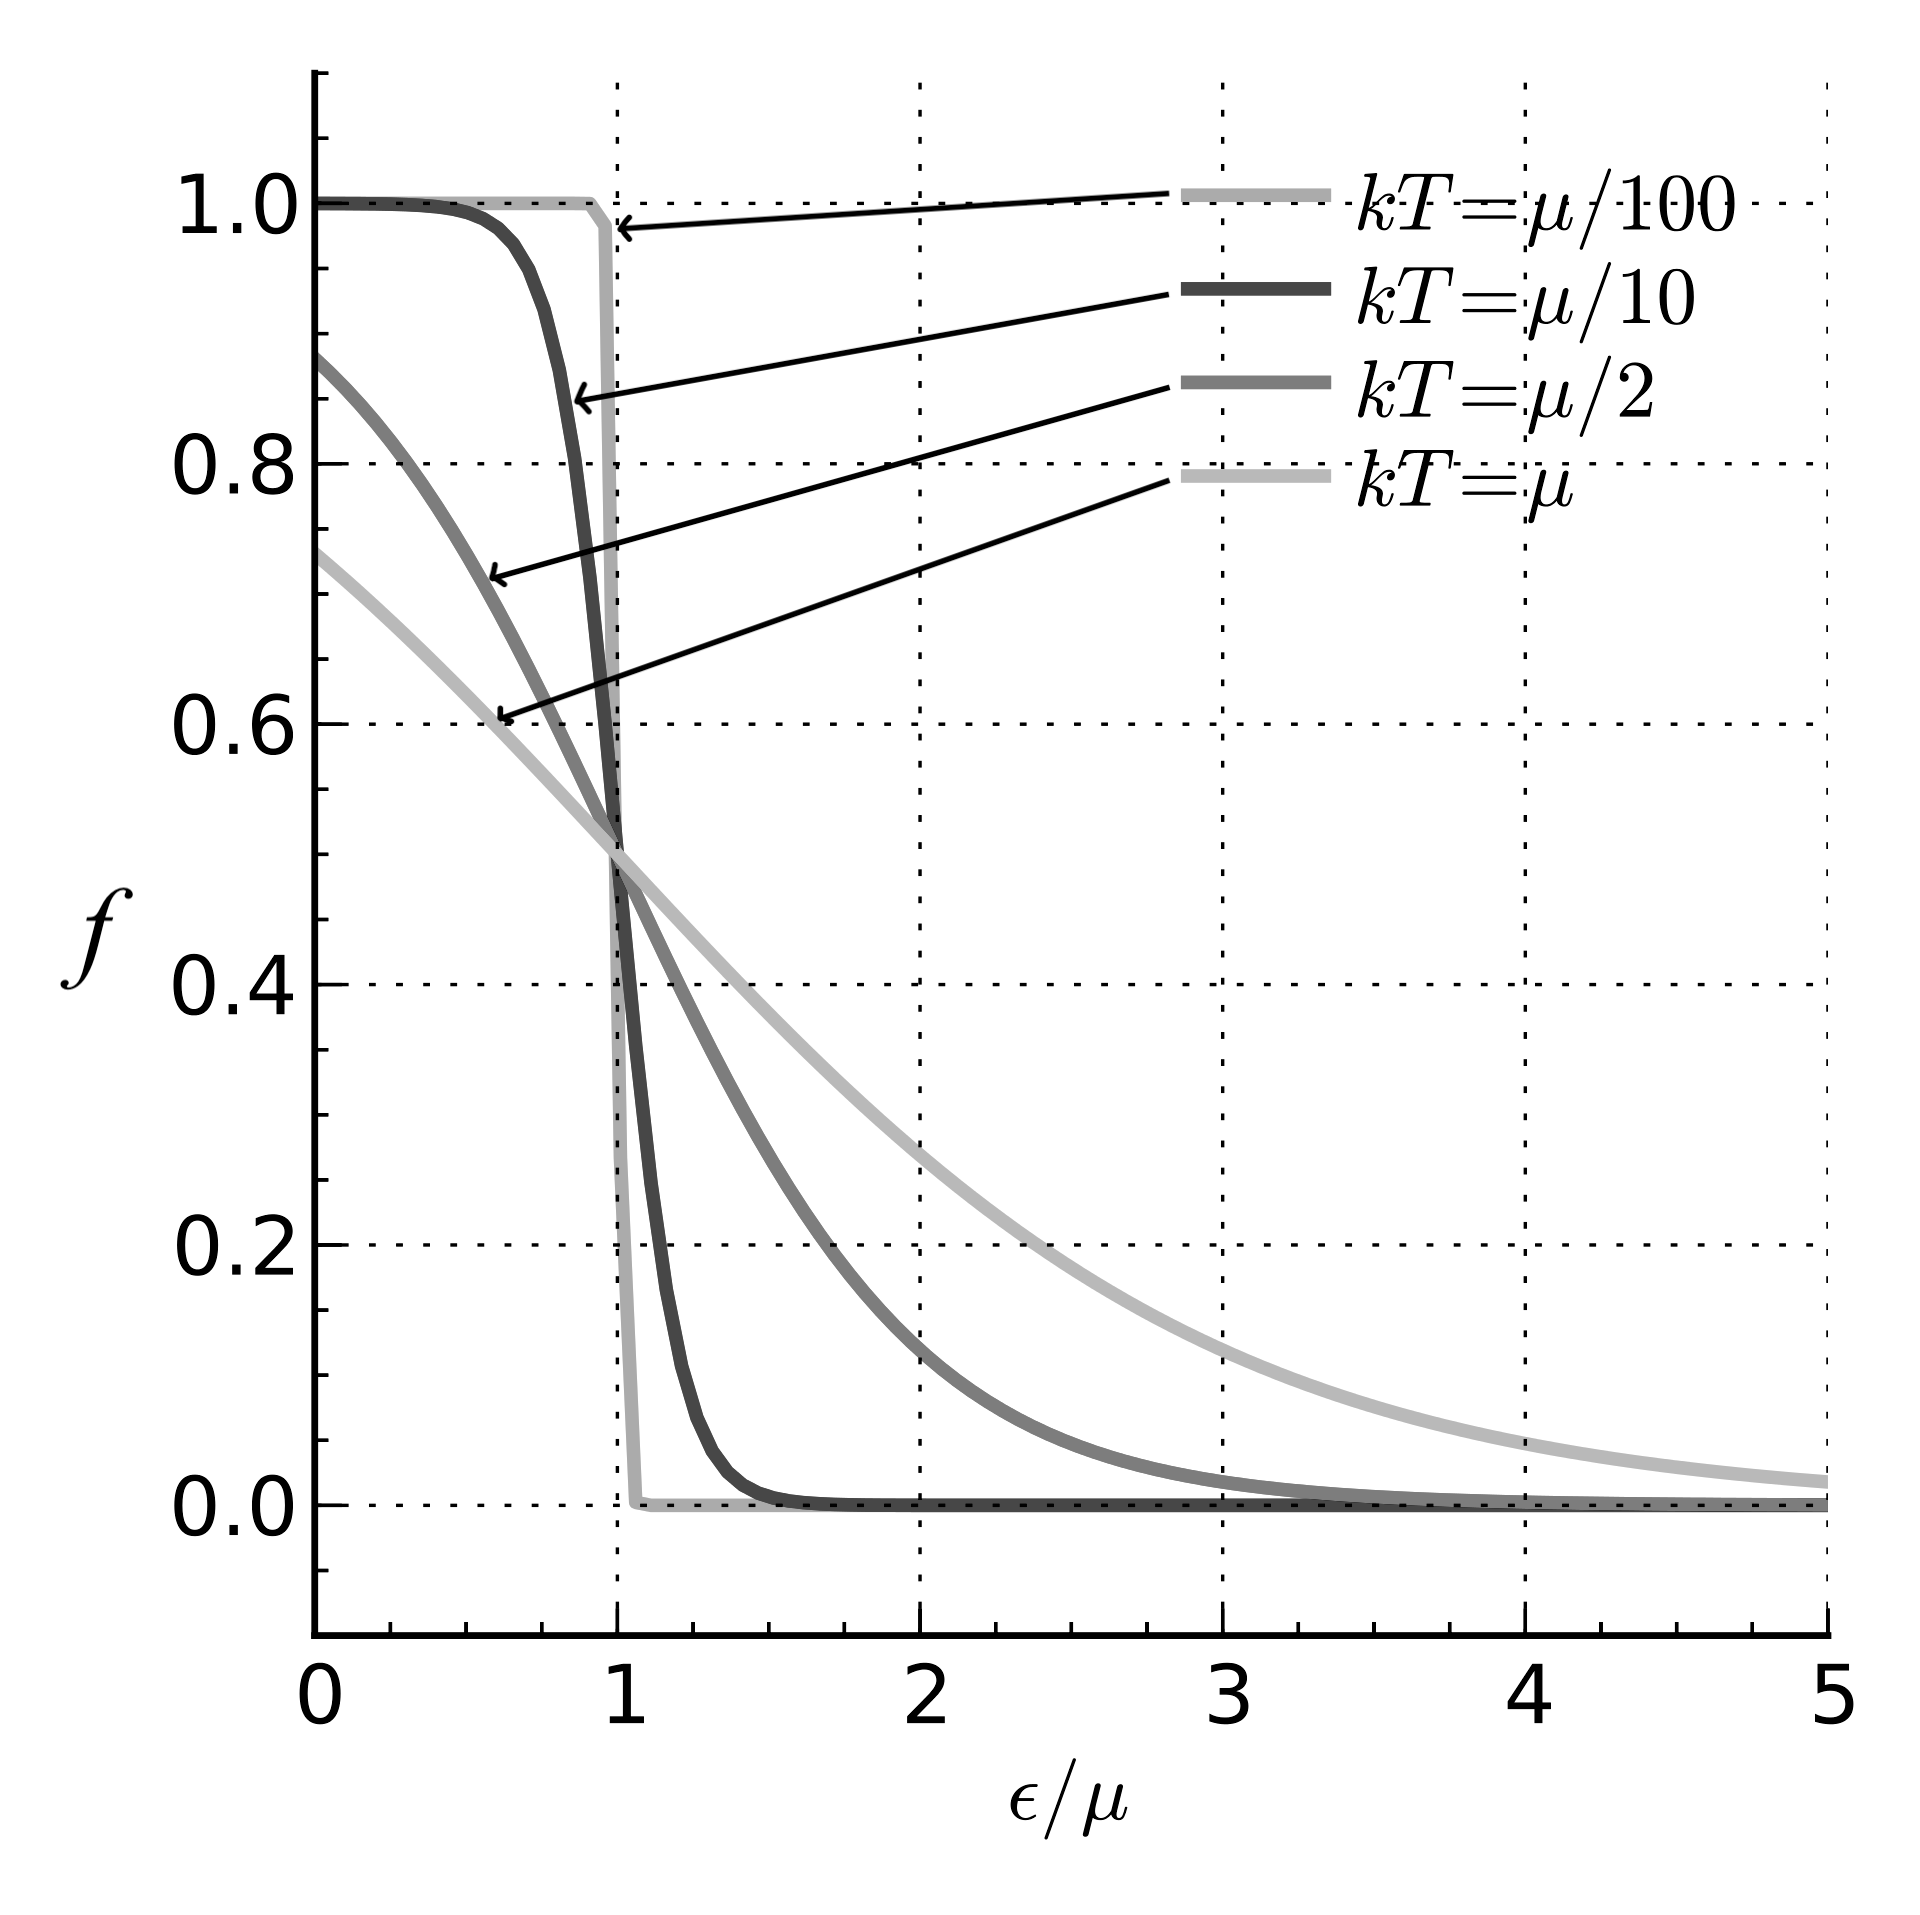
\includegraphics[height = 6cm, width = 7cm]{Fermi}
\end{center}
\begin{center}
Figure 2.2: Graph of $f(\frac{\epsilon_n}{\mu})_{nm}$ vs $\frac{\epsilon_n}{\mu}$
\end{center}
%%%%%%%Graphics

This graph can be interpreted in multiple ways:
\begin{enumerate}
\item The most simple and straightforward interpretation is that in a system in which only one fermion is to occupy any given energy state, the probability of its occupation of an energy state $n$ increases as $\epsilon_n \rightarrow 0$. This is because $p_{(00...100..)} = f_{1}f_{2}...f_{n}f'_{n+1}f'_{n+2}...$ This again provides us with the powerful fact that for a one-fermion-system, the probability of it 'filling' a given state is highest if it is the ground state, i.e the ground state is the most probable.

\item Consider a fermionic system having fixed discrete energy levels $\epsilon_1,\epsilon_2,\epsilon_3....$ in contact with a particle reservoir. Let us say we have no idea of how the fermions are spread out over the energy levels. Given that $f_{nm}$ is a statistical \emph{weight} associated with a given energy level, it leads us to conclude that an energy level having greater 'weight' is more likely to be occupied. This tells us that orbitals with $\epsilon_n < \mu$ have a \emph{greater relative likeliness of being individually occupied.}\\
 This is a very subtle statement, and may not mean much in case of fermions, because we can find the \emph{exact} probability of a particular meta-configuration. However, in the case of bosons, relative probabilities of occupancies of the energy levels lead to interesting phenomena. Thus, the conclusion is that the relative probability of individual occupancy of an orbital (or a 'room) is high if the energy of the orbital is less than a threshold $\mu$.
\item The previous point is better illustrated with the rather vivid imagery involving a particle reservoir in contact with a fermionic system. The particle reservoir has infinite fermions ready and willing to occupy orbitals in the system. Every fermion has a 'choice' to go to a particular orbital. It is just that for all orbitals with energies less than a threshold $\mu$, the fermion is relatively more likely to occupy that orbital. Thus, the whole system would follow a distribution such that the fermions would be highly likely to individually occupy and hence \emph{saturate} the energy levels upto a certain threshold given by 
$\mu$, and the energy  levels above this would be highly improbable and hence sparsely populated.
\end{enumerate}



 \begin{mdframed}[style=exercise]
 \textbf{Summary of Fermi-Dirac Statistics}\\
For a system comprising of fermions, the probability of occupation of a particular orbital (treating the orbital as an isolated system) is called $f_{nm}$, and is given by
\[f_{nm} = \frac{1}{e^{\beta(E_{n} - \mu)}+ 1} \]
This $f_{nm}$ happens to be a statistical weight in the equation 
\[ U = \sum_{n,m}^{}E_{n}f(E_n)_{nm} \]
and \emph{may} be interpreted as 'the probability of occupation of the energy level $E_n$'. This interpretation is used
\begin{enumerate}
 \item To gain additional insight about the \emph{relative} occupancies of the energy levels as $E_n$ and $\mu$ vary. 
 \item To simplify calculations, as it is easier to calculate $\sum E_nf(E_n) $
 \end{enumerate}
 A fermionic system can be solved without alluding to $f_{nm}$ even once.

 \end{mdframed}
 
 
 
\subsection{The Classical Ideal Gas}
It shouldn't be shocking that our notions of what we mean by 'an ideal gas' are those that allow us to conclude that an ideal gas is nothing but a fluid comprising of fermions. It is true that we do not know their spin, and the antisymmetry condition makes no sense. However, the algorithm developed in the previous section does not specifically allude to spin or antisymmetry. The most important detail, that fermions are indistinguishable, gives us enough justification to try to model an ideal gas as a fermionic fluid. \\

In this case, energies are characterised only by the wave number $k$, as given below:

\[ \epsilon_{k,m_s} = \frac{p^2}{2m} =   \frac{\hbar^2k^2}{2m} \]

where m is the mass of a fermionic particle. An orbital is thus specified by $k$ and $m_s$, and this forms our 'subsystem'. This abstract 'subsystem' should be visualised exactly the same way as was visualised in the previous example, similar to different 'rooms' that can either be occupied or unoccupied. The only difference is that in this case, we shall integrate instead of discretely summing up, because $\epsilon$ is a function of a continuous $k$ (as opposed to a discrete $n$), with the density of states being
\[g(\epsilon)d\epsilon = \frac{V}{2\pi^2}k^2dk =  \frac{V}{4\pi^2}\Bigg(\frac{2m}{\hbar^2}\Bigg)^{\frac{3}{2}}\epsilon^{\frac{1}{2}}d\epsilon \]

We obtain the partition function of a subsystem as
\[ z_{(k,m_s)}  = 1 + e^{-\beta(\frac{\hbar^2k^2}{2m}-\mu)} \]
and the Grand Partition Sum as
\[Z_0 = \prod_{k,m_s}{}z_{(k,m_s)} = \prod_{m_s}^{}\prod_{k}^{}z_k = \prod_{k}^{}(z_k)^{(2s + 1)} 
= \prod_{k}^{}\Big[1 + e^{-\beta(\frac{\hbar^2k^2}{2m}-\mu)}\Big]^{(2s + 1)} \]

where $(2s + 1)$ is the number of times each subsystem partition will appear in the product, $s$ being the unknown spin of the fermionic gaseous molecules. We now use $-\beta\Psi = \ln Z_0$ to obtain

\[\Psi = \frac{-(2s+1)}{\beta}\int_{0}^{\infty} \ln\Big[1 + e^{-\beta(\epsilon-\mu)}\Big]g(\epsilon)d\epsilon \]


Integrating by parts, we have

\[\Psi = \Bigg(\frac{-2}{3}\Bigg)\frac{(2s+1)V}{4\pi^2}\Bigg(\frac{2m}{\hbar^2}\Bigg)^{\frac{3}{2}}\int_{0}^{\infty} \frac{\epsilon^{\frac{3}{2}}}{e^{\beta(\epsilon-\mu)}+1}d\epsilon 
=    \Bigg(\frac{-2}{3}\Bigg)\int_{0}^{\infty}\epsilon f(\epsilon) \times (2s+1)g(\epsilon)d\epsilon
\]

where $f(\epsilon)$ is the mysterious probability/weightage factor discussed at great length in the previous section, given as usual by

\[f(\epsilon) = \frac{1}{e^{\beta(\epsilon-\mu)}+1} \]

The relation analogous to $U = \sum\epsilon f(\epsilon)$ in the integral notation, is 

\[  U =  \int_{0}^{\infty}\epsilon f(\epsilon) \times (2s+1)g(\epsilon)d\epsilon \]

which gives us $\Psi = \frac{-2U}{3}$. Using $\Psi = -PV$ we obtain

\begin{center}
\boxed{PV = \frac{2}{3}U}
\end{center}

This is a powerful equation that is true for any fermi fluid. However, to obtain an equation that is specific to the ideal gas, we need to make a particular move that distinguishes any general fermi fluid from a classical gas. The hallmark of the classical regime is that there are relatively few particles distributed over many states. This behaviour is reflected in the quantum regime only when $\mu$ is very low. The relative probabilities of the occupancy of all states with energy greater than $\mu$ is very low, and setting a low $\mu$ would achieve the 'classical' effect that we want. Thus, to describe a fermi fluid that behaves classically, we take $e^{\beta\mu} \ll 1$. This gives us

\[f(\epsilon) \approx e^{\beta\mu}e^{-\beta\epsilon} \]

We write 

\[  N =  \int_{0}^{\infty}f(\epsilon) \times (2s+1)g(\epsilon)d\epsilon =
 \frac{(2s+1)V}{4\pi^2}\Bigg(\frac{2m}{\hbar^2}\Bigg)^{\frac{3}{2}}e^{\beta\mu}\int_{0}^{\infty} \epsilon^{\frac{1}{2}}e^{-\beta\epsilon}d\epsilon 
 \]

and
\[  U =  \int_{0}^{\infty}\epsilon f(\epsilon) \times (2s+1)g(\epsilon)d\epsilon = 
 \frac{(2s+1)V}{4\pi^2}\Bigg(\frac{2m}{\hbar^2}\Bigg)^{\frac{3}{2}}e^{\beta\mu}\int_{0}^{\infty} \epsilon^{\frac{3}{2}}e^{-\beta\epsilon}d\epsilon 
\]
On evaluating the integrals and dividing, we obtain

\begin{center}
\boxed{U = \frac{3}{2}Nk_BT }
\end{center}
which is the glorious, familiar equation for the ideal gas as we know it.\\

One may ask, how Willard Gibbs came up with the Classical Density States way before quantum mechanics was developed. The answer is that he used the following as his partition function:

\[z = A\int\int\int e^{-\beta E(p_x,p_y,p_z)}Vdp_xdp_ydp_z \]

Whether this was a lucky guess, or a stroke of genius, no one can tell. However, we can corroborate his partition function. It is left to the reader to show that $\int\frac{e^{-\beta E(k)}Vk^2dk}{2\pi^2}$ can be reduced to Gibbs' formulation by taking $p = \hbar k$, $4\pi p^2dp$ = $dp_xdp_ydp_z$ and $A = \frac{1}{h^3}$.\\ 

Gibbs' formulation provides an easy proof for \textbf{The Equipartition Theorem}. We consider Gibbs' partition function in terms of a general coordinate $p$. If $E(p)$ is of the form $E = Cp^2$, then we have

\[z \sim \int e^{-\beta p^2}dp = \Bigg( \frac{\pi k_BT}{C}\Bigg)^{\frac{1}{2}}\]
This means that if the energy is a quadratic function of 'p' then this quadratic term contributes to a factor of $T^\frac{1}{2}$ to the partition function. Equivalently, every quadratic term contributes a factor term of $\Big(\frac{1}{2}N\ln T\Big)$ to $-\beta F$ or a term $\Big(\frac{-1}{2}Nk_BT\ln T\Big)$ to the Helmholtz Potential $F$, or a term $\Big(\frac{1}{2}Nk_BT(1+ \ln T)\Big)$ to the entropy $S$. \\

The most powerful version of this statement is that \emph{every quadratic term contributes a term $\frac{1}{2}Nk_B$ to the Heat Capacity}. This is the statement of the equipartition theorem.\\

It allows us to freely say that for a classical gas with three translational degrees of freedom, the energy is quadratic in the momentum in each direction, and therefore, each momentum contributes $\frac{1}{2}Nk_B$ to a total of $\frac{3}{2}Nk_B$ to the heat capacity. Similarly, rotational energies are quadratic in the angular velocity, and each rotational mode contributes $\frac{1}{2}Nk_B$ to the heat capacity. The same goes for the vibrational modes, which are quadratic in the displacement.\\

The only catch is $e^{-\beta E}$ must contribute significantly to the integral, i.e the energy contribution by the degree  of freedom must be of the order of $k_BT$.\\

Finally, the classical \textbf{Maxwell-Boltzmann Distribution} for velocities of the molecules of an ideal gas is obtained as follows: We call the number of molecules per unit volume of the container with velocities between $v$ and $v+dv$ as $n(v)dv$. It is easy to see that if there are a total of $N$ molecules in the container with volume $V$, then we have

\[ n(v)dv = \frac{N}{V}p(v)g(v)dv\]

Here $g(v)dv$ is the density of states, in the 'velocity space' as opposed to the 'k-space'. Just as $g(k)dk$ was calculated, we calculate $g(v)dv$ and it (unsurprisingly) comes out proportional to $v^2$. Also, $p(v)$ is the probability of a particle having velocity $v$, and this is simply given by the canonical $p(v) = \frac{e^{-\frac{mv^2}{2K_BT}}}{Z}$.\\

Overall, the distribution adopts the familiar form
\[n(v)dv = Cv^2e^{-Av^2} \]
which is exactly what the Maxwell-Boltzmann velocity distribution is supposed to be. A rigorous derivation(that has been omitted for the sake of brevity) would include the values of the constants, which can then be used to calculate the most probable velocity, the root mean squared velocity etc.

\subsection{Bose-Einstein Statistics}
The statistical description of bosonic systems is extremely similar to that of fermions. Let us skip the didactic example of a discrete-energy-level system and jump directly to a bose fluid.\\

We consider an orbital to be identified individually by specific constants $k$ and $m_s$, the energy $\epsilon$ being a function of $k$. We consider every orbital to be an isolated subsystem in contact with thermal and boson reservoirs. The partition sum for an orbital is thus

\[z_{(k,m_s)} = 1 + e^{\beta(\epsilon_k - \mu)} + e^{\beta(2\epsilon_k - 2\mu)} + e^{\beta(3\epsilon_k - 3\mu)} +...... = \frac{1}{1 - e^{-\beta(\epsilon_k - \mu)} }\]


We obtain the Grand Partition Sum as

\[Z_0 = \prod_{k,m_s}{}z_{(k,m_s)} = \prod_{m_s}^{}\prod_{k}^{}z_k = \prod_{k}^{}(z_k)^{(2s + 1)} 
= \prod_{k}^{}\Big[\frac{1}{1 - e^{-\beta(\epsilon_k - \mu)} }]^{(2s + 1)} \]

where $(2s+1)$ is the factor introduced due to bosonic spin $s$. We use $-\beta\Psi = \ln Z_0$ to obtain

\[\Psi = {(2s+1)k_BT}\int_{0}^{\infty} \ln\Big[1 - e^{-\beta(\epsilon-\mu)}\Big]g(\epsilon)d\epsilon = \Big(\frac{-2}{3}\Big)\frac{(2s+1)V}{4\pi^2}\Big(\frac{2m}{\hbar^2}\Big)^{\frac{3}{2}}\int_{0}^{\infty} \frac{\epsilon^{\frac{3}{2}}}{e^{\beta(\epsilon-\mu)}-1}d\epsilon \]
\[=    \Big(\frac{-2}{3}\Big)\int_{0}^{\infty}\epsilon \tilde f(\epsilon) \times (2s+1)g(\epsilon)d\epsilon
= \Big(\frac{-2}{3}\Big)U = -PV \]

Here $\tilde f(\epsilon)$ is the boson analogue the fermionic $f(\epsilon)$. $\tilde f(\epsilon)$  also satisfies $N_t = \sum \tilde f(\epsilon_n) $ and $U = \sum \epsilon_n\tilde f(\epsilon_n) $. However, the exact definition of $\tilde f$ is fundamentally different from that of $f$. \\

Unlike fermions, \emph{any number} of bosons can occupy an orbital, and thus it makes no sense to ask what the probability of a boson of occupying a particular orbital is. Instead, it makes more sense to ask what the \emph{mean number of bosons} that occupy an orbital is. We thus define $\tilde f_{k,m_s}$ as

\[ \tilde f_{k,m_s} = \bar n_{k,m_s} \]

where $\bar n_{k,m_s}$ is the mean number of bosons occupying an orbital. Since an orbital is in itself an isolated system, we can sum over all the \emph{states that the orbital can be in}(in terms of number of occupants) and use it to find the mean occupancy:

\[ \bar n_{k,m_s} = \sum_{j}^{} p_jn_j = \sum_{j}^{} \frac{e^{-\beta(E_{j} - \mu n_j)}}{z_{k, m_s}}n_j = \frac{1}{z_{k, m_s}}\Big[ e^{\beta(\epsilon_k - \mu)} + 2e^{\beta(2\epsilon_k - 2\mu)} + 3e^{\beta(3\epsilon_k - 3\mu)} +......         \Big] \]

On evaluating the infinite sum, we obtain

\begin{center}
\boxed{ \tilde f(\epsilon)_{(k,m_s)} = \frac{1}{e^{\beta(\epsilon_k-\mu)}-1}   }
\end{center}

The integral equation

\[  U =  \int_{0}^{\infty}\epsilon \tilde f(\epsilon) \times (2s+1)g(\epsilon)d\epsilon \]

of course provokes us to consider $\tilde f(\epsilon)$ as some sort of 'statistical weight' for the occupation of an energy level having energy $\epsilon$, and we are justified in doing so.\\

However, we are not justified in calling it a 'probability', because a simple analysis of $\tilde f$ would reveal that it can be greater than unity. Moreover, it is defined as \emph{the mean occupation number} of an orbital, and is bound to be more than one. Therefore, we shall simply have to make do with treating it as a statistical factor that accounts for 'the relative likeliness' of a boson from a particle reservoir to move into an orbital with energy $\epsilon$.\\


Let us for a moment consider the equation

\[  N_t =  \int_{0}^{\infty}\tilde f(\epsilon) \times (2s+1)g(\epsilon)d\epsilon \]

As usual, if we do not have a particle reservoir, but the total number of particles in the system is fixed, we can use this equation to find $\mu$ in terms of $N_t$. In all physical cases, where the total number of particles is bounded and where we choose a scale such that the lowest energy orbital has zero energy, we find that $\mu < 0$. If $\mu$ were positive, then the orbital state with energy $\epsilon_k = \mu$ would have an infinite occupation number.\\

However, there are surprising cases in nature where the total number of particles is \emph{not} bounded. An example is a gas of photons in a vessel maintained at a temperature $T$ and having conducting walls. There exist processes, for instance, in which two photons interact through a nonlinear coupling to produce three photons.\\

In such a case, $N_t$ is not fixed and as a consequence we obtain $\mu = 0$, i.e bosons can move freely in and out of the abstract 'reservoir' that the system is considered to be in equilibrium with. $\mu = 0$ does reduce our Grand Canonical Formalism to the simple Canonical Formalism, which is precisely how we have derived the equations for this special example in Section 2.5.3. \\

The Canonical Formalism is thus mathematically equivalent to considering a model of a non-conserved boson gas with $\mu =0$. There is no specific need to adopt this highly contrived model, but Max Planck used it to formulate what is known as \textbf{ The Planck distribution }. The Planck distribution essentially characterises a statistical distribution of non-conserved bosons(especially photons) by using the term $\grave f(\epsilon)$ given by

\begin{center}
\boxed{ \grave f(\epsilon) = \frac{1}{e^{ \frac{\epsilon}{k_BT}}-1} }
\end{center}

This is simply another avatar of $\tilde f$ with the special condition that $\mu = 0$. It gives us the relative likeliness of the occupancy of an orbital having energy $\epsilon$, in a non-conserved boson fluid.\\

Let us return to a conserved bose fluid in which the energy is purely kinetic, i.e as $\epsilon_{k} = \frac{p^2}{2m} =   \frac{\hbar^2k^2}{2m}$. This allows us to calculate the density of states(proportional to $\epsilon^\frac{1}{2}$) and gives us the following:

\[  N_e =  \int_{0}^{\infty}f(\epsilon) \times (2s+1)g(\epsilon)d\epsilon 
= \frac{(2s+1)V}{4\pi^2}\Bigg(\frac{2m}{\hbar^2}\Bigg)^{\frac{3}{2}}\int_{0}^{\infty} \frac{\epsilon^{\frac{1}{2}}}{\xi e^{\beta\epsilon}-1}d\epsilon 
 \]

Where we have used $\xi = e^{\beta\mu}$, and we are calling $N_t$ as $N_e$(for reasons which shall become apparent soon). Since $\mu < 0$ we obtain $0<\xi<1$. \\

A bit of mathematics allows us to expand the integral given above in powers of $\xi$, giving us

\[N_e =  \frac{(2s+1)V}{\lambda_T^3}\Gamma_{\frac{3}{2}}(\xi) \]

where $\lambda_T$ is called the "Thermal Wavelength" of the bosons at temperature $T$, given by

\[ \lambda_t = \frac{h}{\sqrt{2\pi mk_BT}}\]

and $\Gamma_x(a)$ is defined as 

\[\Gamma_x(a) = \sum_{r = 1}^{\infty}\frac{a^r}{r^x} \]

Integrating similarly for $U$, we obtain

\[U = \frac{3}{2}k_BT \frac{(2s+1)V}{\lambda_T^3}\Gamma_{\frac{5}{2}}(\xi) \]

Dividng $U$ by $N_e$, we have

\[U = \frac{3}{2}N_ek_BT\frac{\Gamma_{\frac{5}{2}}(\xi)}{\Gamma_{\frac{3}{2}}(\xi) }
= \frac{3}{2}N_ek_BT\Bigg[\frac{\xi + \frac{\xi^2}{4\sqrt 2} + \frac{\xi^3}{9 \sqrt 3} + ...}{\xi + \frac{\xi^2}{2\sqrt 2} + \frac{\xi^3}{3 \sqrt 3} + ...} \Bigg]
 \]
 
 If we take $\xi \ll 1$, then we go into the classical regime and re-obtain the formula for the ideal gas(which shows us that a classical gas can be modelled as either fermions or bosons, and spin does not matter).\\
 
 However, this derivation is brought to a screeching halt once we notice that $0<\xi<1$ implies $0<\Gamma_{\frac{3}{2}}(\xi)<2.612$. Thus, trying to obtain $\mu$ from the equation $\Gamma_{\frac{3}{2}}(\xi) = N_e \frac{\lambda_T^3}{(2s+1)V} $ may yield \emph{no solution}, for 
 $N_e, \lambda_T, V$ can be chosen such that $N_e \frac{\lambda_T^3}{(2s+1)V} > 2.612$\\
 
This 'error' stems from the fact that we are dealing with special cases of temperatures where $N_e \frac{\lambda_T^3}{(2s+1)V} > 2.612$. Equivalently, for all temperatures less than or equal to $\frac{2\pi\hbar^2}{k_Bm}\Big(\frac{N_e}{2.612(2s+1)V}\Big)^\frac{2}{3}$, we must follow a different approach. This special temperature, given by
 
 \begin{center}
 \boxed{ T_c = \frac{2\pi\hbar^2}{k_Bm}\Big(\frac{N_e}{2.612(2s+1)V}\Big)^\frac{2}{3} }
  \end{center}
  
 is called the \textbf{Condensation Temperature} of the bose fluid. What exactly happens if we take a system below this sharply defined temperature?\\
 
 Going below this temperature increases $\xi$(which gets closer to 1), and hence increases $\mu$(which approaches zero from the left). Thus considering the ground state orbital energy to be some $\epsilon_0 \ll 1$, $\mu$ approaches $\epsilon_0$ from the left. \\
 
Let $n_0$ be the total number of particles in the ground state with energy $\epsilon_0$. $n_0$ is given by

\[n_0 = \tilde f(\epsilon_0) =  \frac{1}{e^{\beta(\epsilon_0 - \mu)}-1}\]

As $\mu$ approaches $\epsilon_0$, it follows that $\beta(\epsilon_0 - \mu) \ll 1$ and consequently $n_0 \gg 1$. We inquire as to what value of $\mu$ results in $n_0$ being equal to the total number of particles $N_t$ present in the system. We obtain

\[ n_0 =    \frac{1}{e^{\beta(\epsilon_0 - \mu)}-1} \sim N_t \implies \beta(\epsilon_0 - \mu) \sim \frac{1}{N_t} \]

If we continue to decrease the temperature $\mu$ would come as close $\epsilon$ as possible, and this would result in the ground state hosting \emph{all} of the $N_t$ particles of the gas. This is precisely what is known as \textbf{Bose-Einstein Condensation}.\\

The mathematical formalism for dealing with this special phenomena involves us calling the total number of particles in the system $(N_t)$ as 

\[ N_t = n_0 + N_e \]

 where $n_0$ refers to the number of particles occupying the ground state, and is given by $n_0 = \frac{\xi}{1-\xi}$. $N_e$ refers to the number of particles occupying the excited states and is given by $N_e = \frac{(2s+1)V}{\lambda_T^3}\Gamma_{\frac{3}{2}}(\xi)$
We choose an energy scale where $\epsilon_0 = 0$ and therefore the total energy of the system as exactly the same as that before, given by $U = \frac{3}{2}k_BT \frac{(2s+1)V}{\lambda_T^3}\Gamma_{\frac{5}{2}}(\xi)$; for ground state occupancy does not contribute to the energy.\\

Finally, we see as that for any $T<T_c$, the maximum number of excited bosons is
 $ N_e =  \frac{(2s+1)V}{\lambda_{T} ^3}\Gamma_{\frac{3}{2}}(1)$.
Particularly, as $T \rightarrow T_c$, $N_e \rightarrow N_t$ giving us 
$ N_t =  \frac{(2s+1)V}{\lambda_{T_c} ^3}\Gamma_{\frac{3}{2}}(1)$.
Dividing, we obtain the powerful relation 
\[ \frac{N_e}{N_t} =\Bigg(\frac{\lambda_{T_c}}{\lambda_{T}}\Bigg)^{3} =\Bigg(\frac{T}{T_c}\Bigg)^\frac{3}{2} \]

Thus, in this formalism, we have the following results:
\begin{enumerate}
\item For $\bm{T>T_c}$, we have 
\[n_0 \ll N_t 
\hspace{0.7cm};\hspace{0.7cm}
N_e \approx N_t = \frac{(2s+1)V}{\lambda_T^3}\Gamma_{\frac{3}{2}}(\xi) 
\hspace{0.7cm};\hspace{0.7cm}
U = \frac{3}{2}N_ek_BT\frac{\Gamma_{\frac{5}{2}}(\xi)}{\Gamma_{\frac{3}{2}}(\xi) }
\]

\item For $\bm{T<T_c}$, we have 
\[ \frac{n_0}{N_t} = 1 - \Big(\frac{N_e}{N_t}\Big) = 1 - \Bigg(\frac{T}{T_c}\Bigg)^\frac{3}{2} 
\hspace{1cm}and\hspace{1cm}
  U = \frac{3}{2}N_tk_BT\frac{\Gamma_{\frac{5}{2}}(1)}{\Gamma_{\frac{3}{2}}(1) } \Bigg(\frac{T}{T_c}\Bigg)^\frac{3}{2}  \]

\end{enumerate}



 \begin{mdframed}[style=exercise]
 \textbf{Summary of Bose-Einstein Statistics}\\
For a system comprising of bosons, \textbf{the mean number of particles occupying an orbital} $\tilde f(\epsilon)_{(k,m_s)} $ is given by \[ \tilde f_{(k,m_s)} = \frac{1}{e^{\beta(\epsilon_{k} - \mu)} - 1} \]
This $\tilde f_{(k,m_s)}$ happens to be a statistical weight in the equation 
\[  U =  \int_{0}^{\infty}\epsilon \tilde f(\epsilon) \times (2s+1)g(\epsilon)d\epsilon \]
and \emph{may} be interpreted as 'the relative likeliness' of a boson from a particle reservoir to move into an orbital with energy $\epsilon_k$.\\ \\


 \end{mdframed}


%%%%%%%%%%%%%%%%%%%%%%%%%%%%%






























%%%%%%%%%%%%%%%%%%%%%%%%%%%%%
\chapter{The Laws of Thermodynamics}
\section{The Zeroth, First and Third Laws}
The Zeroth Law of thermodynamics states that,\emph{"If two systems, A and B, are separately in equilibrium with a third system, C, then they are also in equilibrium with one another"}. This law follows directly from the definition of Temperature, and a sketch of its proof is present in Section 1.4.\\

The First Law states that, \emph{"The amount of work required to change the state of an otherwise adiabatically isolated system depends only on the initial and final states, and not on the means by which the work is performed, or on the intermediate stages through which the system passes"}.\\

Closer inspection of this statement reveals that it is nothing more than a restatement of the Energy Conservation Principle. Let the amount of work done to take a system adiabatically from one state to another  be $W_1$ in one case and $W_2$ in another, such that $W_1>W_2$. The obvious question that would arise, would be \emph{"Where does the extra energy put in doing the work $W_1$ go?"} Thankfully, the Energy Conservation Principle assures us that the energy of any isolated system is conserved, and considering the universe to be an isolated system, the total energy of the universe is conserved. Therefore, $W_1$ \emph{must} equal $W_2$.\\

 Even if we do not consider the process to be adiabatic, we \emph{define} heat in such a way that it accounts for unknown modes of a system that might consume energy. Thus, in any process, the change in energy is equal to the heat flux to the system and the work done on the system, during that process.\\

Like other conservation principles, the roots of the Energy Conservation Principle lie in Noether's Theorem. The constancy of the energy of an isolated system, is merely a consequence of the symmetry of the dynamical laws governing that system, under time translation. Even if we are to avoid delving into Group Theory, energy conservation (and equivalently, the first law of thermodynamics) is a very natural principle that we have been born and brought up with, and doesn't require much explanation.\\

The Third Law of thermodynamics states that, \emph{"The entropy of all systems at absolute zero  temperature is a universal constant that can be taken to be zero".} The Third Law is often called 'The Nernst Postulate', and it is exactly the same as the fourth postulate that we have defined in Section 1.3.\\

Unlike the other laws, the Third Law is not integral to the structure of the rest of thermodynamic theory, and its implications become clear only in the low temperature regions where $T \rightarrow 0$. Since we do not encounter near-zero Temperatures in most of Physics, it is best to accept it without much ado.\\

 Another restatement of the third law is that, \emph{"The $T=0$ adiabat is coincident with the 
$S = 0$ isentrope".} Since the $T=0$ adiabat does not intersect any other adiabat, a corollary that follows is: \emph{"No reversible adiabatic process starting at a non-zero temperature, can possibly bring a system to zero temperature".} The question of whether the \emph{absolute zero} of the temperature can be achieved by \emph{any} process, is a rather philosophical one, and it deals with us having to ponder over what it means for a system to be 'truly isolated'. We are of course, also quantum mechanically limited in the precision that we can achieve in the measurement of any physical quantity. 

\section{The Second Law}
Here are some of the different 'avatars' of the Second Law:
\begin{enumerate}
\item \textbf{Kelvin’s statement} "No process is possible whose sole result is the complete conversion of heat into work."
\item \textbf{Clausius’s statement} "Heat cannot flow spontaneously from a material at a lower temperature to a material at a higher temperature."
\item \textbf{Engine statement} "The efficiency of a Heat Engine can never be unity."
\item \textbf{Refrigerator statement} "The efficiency of a Refrigerator is always finite."
\item \textbf{Entropy Statement} "In any thermodynamic process, the total entropy either increases or remains constant, but never decreases."
\end{enumerate}

We have had sufficient motivation(both statistically and phenomenologically) to take the fifth statement to be true. It is nothing but our familiar Entropy Maximisation Postulate.\\

The Engine Statement is equivalent to Kelvin's statement, for if there were a perfect engine, it would be able to extract heat from a reservoir and deliver all of it as work(see Section 1.8). Similarly, Clausius's Statement is equivalent to the Refrigerator Statement, because the impossibility of an ideal refrigerator rules out a process whose sole result is the transfer of heat from a colder body to a hotter body.\\

Consider a perfect engine that violates Kelvin's statement. Let us say this engine extracts heat $Q'$ from a reservoir at temperature $T_H$, and converts all of it entirely to work $W$. Let us couple this engine with a regular pump, that has extracted heat $Q$ from a reservoir at temperature $T_C$. Now the pump functions as it normally would, i.e it does work $W(=Q'$, provided by the perfect engine) on the working substance of the pump, and ejects heat $Q+W = Q+Q'$ into the hotter reservoir $T_H$.\\

Closer inspection of this (perfect engine + normal pump) reveals that it produces exactly the same effect as extracting heat $Q$ from a colder reservoir and releasing it to a hotter reservoir, i.e it behaves like an ideal refrigerator, as shown below:

%GRAPHICSSSSSSSSS
\begin{center}
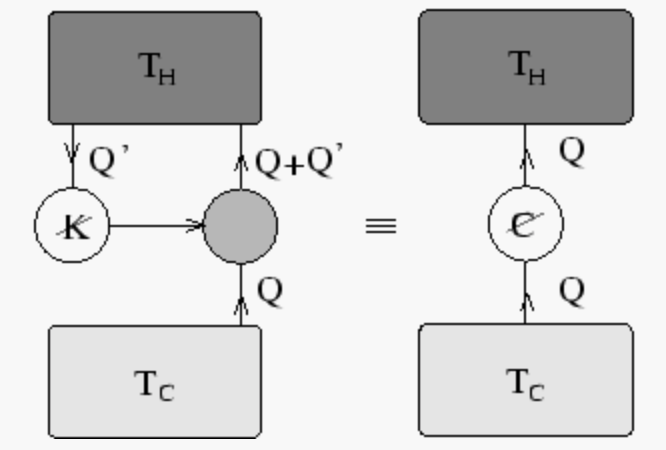
\includegraphics[height = 6cm, width = 9cm]{Buz}
\end{center}
\begin{center}
Figure 3.1: A schematic diagram establishing the equivalence of an ideal engine and an ideal refrigerator,\\
taken from \texttt{https://theory.physics.manchester.ac.uk/$\sim$ judith/stat$\textunderscore$therm/node19.html} 
\end{center}
%%%%%%%%

This ties together the first four statements. If we prove the truth of either one of these statements, then we are done. The way we do this is by making the following claim: If one believes the Entropy Maximisation Postulate, then this postulate does not allow for the existence of a perfect engine.\\

Why is this the case?\\

Let us hark back to the Maximum Work Theorem developed in Section 1.8. This theorem, and its resultant engine efficiency, have both been derived from scratch using only the Entropy Maximum Postulate, and therefore should be viewed as an extension of our four phenomenological postulates. If an engine were to be perfect, it would imply $T_{c} = 0$ which \emph{cannot} be the case. One may justify this using the philosophical unattainability of zero temperature, or using the more mature argument made using the Nernst Postulate, saying that $T_c = 0$ implies the entropy of the cold reservoir to be zero, which would not allow any reversible exchange of heat with a hotter body.\\

In any case, we have proven the equivalence of the five statements of the second law. However, whenever anyone talks about the Second Law, they are more often than not referring to the Entropy Maximisation Postulate.\\

It is here that we state once and for all, that the Second Law \emph{can not be proven}. Entropy Maximisation is a \emph{postulate} that we assume, and motivations for the same have been provided throughout this text. More discussions on these motivations will be made in Section 3.3. Before we move ahead, it is worth mentioning a few incorrect attempts made at 'proving' or 'disproving' the second law, as they represent interesting thoughts that are worth pondering over.\\

Over the decades, people have claimed that Darwinian Evolution violates the Second Law of Thermodynamics. It is claimed that organisation of life-forms leads to a decrease in disorder, and this is a decrease in entropy. Such incorrect arguments stem solely from the fact that 'disorder' is misinterpreted. However, arguments in favour of evolution that rely on stating that organised life-forms have a greater number of 'states' that they can be in, are also not correct. Simple calculations can be done on the (earth+sun) system, by treating both of them as material bodies, and dealing only with their macroscopic, material coordinates. Using these, one can easily prove that the \emph{net} entropy of the earth-sun system always increases, and therefore, any process on earth can't possibly be violating the Second Law.\\

This is an important point. The Second Law does not state that entropy of some part of a system can not decrease. Instead, it claims that a decrease in entropy in a system is followed by a gain in entropy in another connected system, such that the \emph{net} entropy increases. It is easy to verify that for interstellar gaseous clouds that condense into planets and other heavenly bodies, the entropy of the gas clouds \emph{does} decrease, but it is also accompanied by a greater increase in the entropy of some other part of the universe. It is interesting to ponder over \emph{where} the entropy increases, and this is left to the reader as an exercise.\\

Just like Darwin's Theory of Evolution, the Second Law is founded on belief, and is supported by observations. However, many incorrect ideas are used to arrive at these beliefs. The most popular (and incorrect) train of thought is that the increasing entropy of an isolated system is equivalent to claiming that "systems move from less probable states to more probable states", or that entropy increases only because it is 'far more likely to increase than decrease'. \\

Let us open a jar filled with gas molecules, in a big room. The molecules spread out into the room and occupy more states, thereby increasing the entropy. The people who argue for the probabilistic nature of entropy increase, would say: "This is simply because, if the molecules were given a choice to occupy any of the positions in the room, the collective configuration corresponding to them being huddled together in the jar is very less, whereas the probability of any state where the molecules are spread out is more."\\

The problem with this logic is that all the laws of physics are supposed to be symmetric with respect to time translations. Let us consider two molecules in empty space moving towards each other, colliding, and then moving in different directions. If we reverse the direction of time, and reverse the labels of 'left' and 'right', we would observe them moving towards each other, colliding, and moving in different directions again, i.e the 'reverse movie' is symmetric to the 'normal movie'. This is known as the CPT invariance of dynamical laws. In essence, molecules escaping a jar and spreading out is nothing but dynamical laws applied to many, many gaseous particles.\\

However, if we reverse the velocity of every gaseous particle that has escaped the jar and reverse 'left' and 'right', the entire system will exactly retrace its trajectory, and gaseous molecules that were spread out, come and settle back in the jar. At any earlier point in time when the jar was still open, it was incredibly unlikely that all the molecules just happened to be inside the jar. So the system moves from a more probable state to a less probable state,  “proving” that entropy tends to decrease. This brings out the flaw in the 'probabilistic argument' to justify that entropy increases.\\

Early in his career, even Boltzmann made similar probabilistic arguments. The rebuttal to this attempt at 'proving' the second law came from Josef Loschmidt, and it requires us to start with a system in a low entropy (non-equilibrium) state. Given enough time, it will eventually move to a higher entropy, equilibrium state. Reversing the velocity of every particle, the equations of motion being time symmetric, the system will retrace its trajectory and return to the original, low entropy state.\\


During those days, this led to the popular belief that the second law was not a universal law that applied in all cases, because of the counter-example(presented by Loschmidt) where the entropy spontaneously decreases. Boltzmann also ended up recognising that symmetry violations would render the second law 'unprovable' by \emph{any} mechanism. How then, are we to view thermodynamics?\\

The correct interpretation is given here:

\begin{mdframed}[style=exercise]
The Second Law of Thermodynamics is not really a “law” at all. It is a definition. When we speak of “forward in time,” we really mean “the direction of increasing entropy.” 
\end{mdframed}

Cosmological models add greater meaning to this statement and link the uni-directional nature of time to the uni-directional nature of entropy. However, these are far outside the scope of this text.\\

A very important point, which is often lost in translations and textbooks, is that \emph{there are no laws in science.} Throughout this text, we have avoided alluding to the classical 'Laws of Thermodynamics' as they are generally presented in textbooks. This is to reiterate the point that every theory is based on postulates. It just so happens that the postulates of thermodynamics are so natural, that people simply can not believe that there \emph{could exist} phenomena that could go against them.\\

Over the centuries, many varied perspectives of looking at the universe have been in and out of fashion and yet the essential structure of thermodynamics has remained the same. It started off as a set of empirical laws dealing with specific systems like engines. It has since been expanded to cover the widest range that one can imagine. We shall see in the final section of this text how the postulates of thermodynamics are based on two simple principles: some call these principles as observations, while others call them beliefs.\\
 
Irrespective of what one calls them, thermodynamics should be treated like any other scientific theory - it is only a model of the universe. It would be incorrect and frightfully arrogant for any human to define \emph{laws} about how the universe will function even after we are gone. Therefore, thermodynamic laws should be seen not as laws, but as extensions of the postulates. If in the future, these 'laws' are violated, we may need to modify our theory superficially.\\

However, it could also mean that \emph{perhaps our postulates are wrong}. Many great minds have spoken endlessly about why they have immense faith in the validity of the thermodynamic postulates, and why they are confident that even if one may have to modify the structure of the theory in the future, the foundational postulates would never be overthrown.\\

It is indeed risky to call any scientific postulate infallible, and arguments from both sides adopt a philosophical and quasi-religious demeanour. We shall nevertheless explore the basis of the immense confidence and support that is enjoyed by thermodynamic theory, in the coming section.


\section{The Thermodynamic Perspective}
As iterated recently, any theory is like Thermodynamics. There are postulates which one \emph{has to believe}, irrespective of whether on likes them or not, and then the rest of the theory is developed based on these. There are many theories that explain the working of different systems in the universe, and \emph{any theory} that agrees with experiments is accepted.\\


Why is it that thermodynamics is loved above others?\\

The popularity of thermodynamic theory comes from the wide range of its applications, but its true beauty stems from the simplicity of its foundational tenets. The basic postulates are so \emph{natural}(unlike those presented by, say, Quantum Mechanics) that one can't help but \emph{believe} them. These foundational tenets, broadly speaking are the first two laws of, i.e the Energy Conservation Principle and the Entropy Maximisation Postulate.\\

The first law is easy to believe, the second, not so much. If you believe the second law, good. I most certainly didn’t when I read it for the first time.\\

It is easy to observe that the second law is simply a mathematical formulation of the Equilibrium Postulate (Postulate I) developed in Chapter 1. It hinges on one crucial observation about the unidirectional nature of what we call 'spontaneous' and 'non-spontaneous'. What if our observation is wrong? There are many situations in which our 'intuition' is wrong (Quantum Mechanics, is an example). What if we simply haven't waited long enough for a mixture of lemonade and water to 'unmix'?\\

Well, all of science is like this. We observe, and then we postulate. If one believe the observation about the evolution of systems towards equilibrium, (which is far more closer to our heart than the archaic statements of some of the variants of the Second Law), then great. But let us go one step further. Let us say one does not believe that a system will evolve to equilibrium \emph{at all}, and that in the future the system can be in any random, arbitrary state.\\

This is where the statistical mechanical perspective comes into play. We \emph{agree} that in the future the system can be in any random, arbitrary state. We then proceed to adopt a strategy for optimal prediction. Even in this case, all of thermodynamic theory can be developed independently, from scratch. It just so happens that this strategy of optimal prediction involves the maximisation of a function. \\

If one believes in the maximisation of this function, then one \emph{might as well} shake hands with the 'relatively naive' bunch of observational scientists who have developed thermodynamic theory over centuries and have themselves been empirically maximising a function all along. The mathematical exercise of maximising a function, goes hand in glove with the empirical observation of systems evolving unidirectionally towards equilibrium. \\

Thus, we see that the statistical mechanical approach heuristically justifies the phenomenological postulates, which are in themselves quite simple and natural to believe. Even the bitterest cynic would be satisfied with the statistical approach of maximising disorder. (It is to be noted that viewing entropy maximisation as a strategy of optimal prediction is a very modern school of thermodynamics. Classical statistical mechanics was slightly different, but was the same mathematically)\\

Therefore one can view Entropy as one likes it - as a super function that is obtained observationally and empirically, or as a function that characterises our uncertainty about predictions. Most people view it as both, and the modern perspective is to fuse the two different approaches into one unified Entropy, that explains the universe in a simplistic way like no other function does. 


\begin{mdframed}[style=exercise]
This leads us to conclude that the two foundational tenets of Thermodynamics should be, in very loose terms, \textbf{the conservation of energy} and \textbf{the maximisation of uncertainty}.
\end{mdframed}
 
These two principles seem so natural, so simple and so \emph{obviously true}. They are so visceral that any person would be willing to take the risk of calling them infallible. \\

This is why thermodynamics occupies a special place in or hearts. It is the mysterious Black Monolith of Physics, engraved in history, and unlikely to be challenged.  No wonder the greatest physicists of the past century have been absolute masters of statistical mechanics. \\






    
  %%%%%%%%%%%%%%%%%%%%%%%%%%%%%
   
    
\begin{thebibliography}{9}

\bibitem{Thermodynamics and an Introduction to Thermostatistics} 
Herbert B. Callen.
\emph{Thermodynamics and an Introduction to Thermostatistics}
John Wiley \& Sons, Inc.

\bibitem{einstein} 
F. Reif.
\textit{Fundamentals of Statistical and Thermal Physics}
McGraw-Hill Book Company

\bibitem{lol} 
Mehran Kardar
\textit{Statistical Physics of Particles}
Cambridge University Press

\bibitem{knuthwebsite} 
Lecture notes present at
\texttt{http://www.web.stanford.edu/$\sim$peastman/statmech}



\end{thebibliography}
    
  %%%%%%%%%%%%%%%%%%%%%%%%%%%%%
   
    
    
 %%%%%%%%%%%%%%%%%%%%%%%%%%%%%
\end{document}